\documentclass{article}

% *****************************************************************
% Estout related things
% *****************************************************************
\newcommand{\sym}[1]{\rlap{#1}}% Thanks to David Carlisle

\let\estinput=\input% define a new input command so that we can still flatten the document

\newcommand{\estwide}[3]{
		\vspace{.75ex}{
			\begin{tabular*}
			{\textwidth}{@{\hskip\tabcolsep\extracolsep\fill}l*{#2}{#3}}
			\toprule
			\estinput{#1}
			\bottomrule
			\addlinespace[.75ex]
			\end{tabular*}
			}
		}	

\newcommand{\estauto}[3]{
		\vspace{.75ex}{
			\begin{tabular}{l*{#2}{#3}}
			\toprule
			\estinput{#1}
			\bottomrule
			\addlinespace[.75ex]
			\end{tabular}
			}
		}

% Allow line breaks with \\ in specialcells
	\newcommand{\specialcell}[2][c]{%
	\begin{tabular}[#1]{@{}c@{}}#2\end{tabular}}

% *****************************************************************
% Custom subcaptions
% *****************************************************************
% Note/Source/Text after Tables
\usepackage{verbatim}
\newcommand{\figtext}[1]{
	\vspace{-1.9ex}
	\captionsetup{justification=justified,font=footnotesize}
	\caption*{\hspace{6pt}\hangindent=1.5em #1}
	}
\newcommand{\fignote}[1]{\figtext{\emph{Note:~}~#1}}

\newcommand{\figsource}[1]{\figtext{\emph{Source:~}~#1}}

% Add significance note with \starnote
\newcommand{\starnote}{\figtext{* p < 0.1, ** p < 0.05, *** p < 0.01. Standard errors in parentheses.}}

% *****************************************************************
% siunitx
% *****************************************************************
\usepackage{siunitx} % centering in tables
	\sisetup{
		detect-mode,
		tight-spacing		= true,
		group-digits		= false ,
		input-signs		= ,
		input-symbols		= ( ) [ ] - + *,
		input-open-uncertainty	= ,
		input-close-uncertainty	= ,
		table-align-text-post	= false
        }
\usepackage{booktabs}

\usepackage{amsmath,amsthm,amssymb} %Misc math symbols
\usepackage{mathtools}
\usepackage[utf8]{inputenc}
\usepackage[margin=1in]{geometry}
\usepackage{caption} 				%Inserting multiple figures
\usepackage{subcaption}
\usepackage[svgnames]{xcolor}
\usepackage{listings}
\usepackage{tikz, pgfplots} 			%Drawing pictures
\usepackage{fancyhdr} 				%Header style
\usepackage[svgnames]{xcolor}		%Coding styles
\usepackage{enumitem}				%Enumerating using letters
\usepackage{mathrsfs}				%Fonts
\usepackage{listings}
\usepackage{hyperref}
\setlength{\headheight}{15.2pt}
\pagestyle{fancy}
\lhead{ \fancyplain{}{Andrew Kao} }
\rhead{ \fancyplain{}{Winter 2019} }
\chead{ \fancyplain{}{Honors Econometrics: Replicating Leigh 2008} }

\begin{document}

\section{Introduction}

Are American governors ideological? That is, do Democrat and Republican governors differ by the policies they implement, or the outcomes they deliver to their states? Leigh 2008 attempts to answer this broad question by looking at whether a multitude of outcomes differ under Democrat or Republican governorships in a panel extending over 60 years and all 50 states. 

This question has far-reaching consequences, given the considerable effort and investment placed into the political process, and that democracy only credibly functions when voters are able to meaningfully select for policies/outcomes in their interest.

This paper aims to separate two strands of theory in the political economy literature. One, advanced by Downs (1957) characterises candidates and parties as only caring about political victory, with party ideology only relevant insofar as it leads to electoral success. The other, proposed by the likes of Wittman (1973) and Dixit and Londregan (1998) model parties as having exogenous policy preferences and ideology, with later work by Dhami (2003) and Roemer (2001) using intra-party politics (different factions competing) to endogenously generate ideological preferences.

Empirically, Alesina and Rosenthal (1995) have found that Democratic presidents lead to higher growth and higher inflation. On the state level, Plotnick and Winters (1985) and Dilger (1998) both find that partisanship does not impact tax and expenditures, while Reed (2006) finds that Democrats are more likely to raise taxes.


\section{Empirical Strategy}

The paper uses a standard OLS, using the following specification:

\[ Y_{it} = \alpha + \beta G_{it} + \chi_{it} + \epsilon_{it} \]

where $Y$ is the outcome in state $i$ and year $t$, $G$ is a dummy variable for whether the state has a Democratic governor, $\chi_{it}$ is a vector of demographic and political controls indexed by state and year, and $\epsilon_{it}$ a normally distributed error term clustered on the state level.

Depending on the specification, $\chi_{it}$ may contain controls for which party controls the state's legislative chamber, the share of the vote received, the partisanship of the state's representatives in Congress (as measured by Poole-Rosenthal scores), log population of the state, population under age 15, population over age 65, population that is black, and fixed effects for state and year. 

\subsection{Assumptions}

In order for the multiple linear regression model to hold, several assumptions need to hold true.
\begin{enumerate}
\item \textbf{The model is linear in parameters.} This may not be true in the case of every single outcome, but is ameliorated by two factors: first, that it is linear in the independent variable of interest, the party of the governor, since it is an indicator variable and hence a linear trend can be found between means. Second, we can always interpret the coefficients as the best linear approximation.

\item \textbf{Random sampling.} Given that we have the entire relevant population, which is every governor in every state prior to the year 2004, random sampling is not an issue, except in the case of missing outcome variables. However, since outcome variables only tend to be missing in years where they were not collected (typically earlier years), this should not introduce bias that would disrupt the internal validity of the claims.

\item \textbf{No perfect collinearity.} The covariates mentioned above are never perfectly collinear, so this is not a concern. 

\item \textbf{Zero conditional mean.} This is the least credible assumption, as the OLS model alone cannot account for all potential sources of endogeneity. Some concerns can be addressed with the simple OLS, as unlike the share of seats won by a party in a legislative chamber, a governor with 51\% of the vote is not more meaningfully constrained in capability than one that has won 91\% of the vote. However, if governors of different parties do behave differently (or are simply perceived to behave differently), and if voters vote rationally, then such voters would try to elect governors of a specific party in anticipation of economic or social conditions that may require different responses - this would create an issue of reverse causality. The regression discontinuity approach described below makes identification of causality more credible.

\item \textbf{Homoskedasticity.} The Breuch-Pagan test is employed for all outcomes of interest with results displayed in Tables ~\ref{table:bp_outcome} to ~\ref{table:bp_index}. Though homoskedasticity is not always rejected for $p < .1$ when an indicator for governor party is the sole independent variable, it is always rejected once other controls are added in. Thus, all regressions are run using robust standard errors, to correct  for the concern of heteroskedasticity.

\item \textbf{Errors are normally distributed.} This might not hold in the data. However, given that $n \approx 3000$ for most regressions (different outcomes are missing for different observations), large sample inference is valid for the data, so that assumptions regarding normality hold as we approach the asymptotic limit.
\end{enumerate}


\subsection{Regression Discontinuity and Endogeneity}

To control for potential sources of endogeneity, Leigh adopts a regression discontinuity approach, where the discontinuity is based around the margin of victory by which the governor wins.

Given the randomness present in the voting process, it is plausible that governors who barely win the majority vote are similar to those who barely lose it, and so this would act as a quasi-experiment wherein the error should be uncorrelated with the independent variable of interest, the governor's party. 

The regression discontinuity specification is identical to that of the OLS above, except that the sample is further constrained to those with close elections. In Leigh 2008, "close" is defined to be governors that win by a margin of 60\% or less (so a candidate winning 80\% of the popular vote would be on the borderline for inclusion). This appears insufficient to me, as governors that win with 80\% of the vote can look very different from those that barely lose the voter; moreover, the issue of reverse causality can only be credibly rejected when the margin of victory is within the margin of error surrounding election predictions (typically no more than 10\% for polls).

As part of an extension, I narrow these bounds to 10\% (so 55\% or less of the popular vote) and 2\% (so 51\% or less of the popular vote); the latter runs into power issues discussed beneath.

Additionally, since the first year of a governor's term may be impacted by residual policies and effects of the prior governor, which is potentially a source of endogeneity if voters elect retributively (i.e. voters elect a new party into power to punish the prior party for doing poorly), regressions are replicated both omitting and keeping data from the first year of a governor's term.


\section{Data}

The data used in this replication comes directly from Leigh's website, located at \url{http://www.andrewleigh.org/research.htm#PoliticalEconomy}. My attempt to reconstruct the dataset was only partially successful, as though data such as that regarding governors was accessible (and did match Leigh's work), many of the outcomes of interest were hosted on websites or other data sources that are no longer accessible.

Given that the paper aims to answer whether there are differences between governors of different parties, and governors could potentially create change along many axes, a large battery of variables are used for outcomes in this analysis. Present in Leigh's analysis are five categories of variables, and I add in the two final ones to extend on the paper. They are:
\begin{itemize}
\item Political variables and controls
\item Policy settings
\item Intermediate outcomes
\item Social welfare measures - income and income distribution
\item Social welfare measures - work, education, crime, and suicide
\item Abortions
\item PCA Indices
\end{itemize}

Descriptive statistics for all of them are presented in Table ~\ref{table:summary_long}

\subsection{Political Variables and Controls}

Democrat governor, Democrat legislature and their interaction are all dummies. Voteshare received by Democratic Candidate. These variables are sourced from ICPSR (1995) with more recent figures from the Congressional Quarterly database. 

Poole-Rosenthal scores come from Poole's website, range from -1 to 1 (representing liberal to conservative), and are imputed every other year when no election took place.

Demographic information comes from IPUMS, with interpolation used for non census years, while population figures come from the BEA.


\subsection{Policy Settings}

Top income tax and corporate tax rates come from the World Tax Database at the Ross School of Business.

The Tax Redistribution Index and Average Tax Rate are calculated using data from the March 1990 CPS (Current Population Survey), and and involves computing the amount by which the income taxation system reduces the gini coefficient; the specific method is outlined in Leigh 2005, but broadly speaking involves linking respondent incomes to match overall state moments after factoring in various tax policies, and the tax burden then calculated for each state and year. 

Minimum wage data comes from Neumark and Nizalova 2007.

The maximum welfare amount is the most real benefit a family of four can receive under AFDC/TANF.

State employment and salaries are from the BEA.

\subsection{Intermediate Outcomes}

Data on unionization rates are based on the CPS Outgoing Rotation Group (ORG) earnings files, the BLS publication, Directory of National Unions and Associations, and record the percentage of each state's non-agricultural wage and salary employees that are union members.

The incarceration rate statistics are from the Bureau of Justice Statistics, and count the number incarcerated in state prisons per 100,000 people per year.

The execution rates are from Espy and Smykla 2004 and is the execution rate per 100,000 people per year.

Data on transfers, unemployment insurance, state tax revenue and overall state revenues are from the BEA, and in logs where indicated.

\subsection{Social welfare measures - income and income distribution}

Average income, inequality, and poverty measures are calculated from the CPS data, where family incomes are adjusted by dividing by the square root of the family size/individual data is weighted by person-weights to match demographic compositions. Family incomes less than 1/10 and over 10x the median are recoded to those values. Data for poverty in earlier years comes from Unicon.

\subsection{Social welfare measures - work, education, crime, and suicide}

Unemployment rates come from the Bureau of Labor Statistics.

The National Assessment of Education Progress (NAEP) scores are from the National Center of Education Statistics, with four grade scores used because they are the most complete across states and years.

Property and violent crime rates are from the Bureau of Justice Statistics, using crimes committed per 100,000 people per year.

Suicide rates are from Stevenson and Wolfers 2006, where the rate is suicides per 100,000 people per year.

\subsection{Abortions}

First, why look at abortions as an extension to the original paper? Many of the outcomes listed above are not particularly ideological in nature - everybody wants to see lower unemployment rates, or students performing better, or higher incomes. For issues that do have partisan leanings, such as tax rates, it is unclear that voters would be galvanized to actually vote based on partisan splits in policy given their uninspiring nature.

Thus, if the purpose of the paper was to examine to extent to which governors are ideological, then it would make sense to look at outcomes that are the most ideologically divisive. According to Gallup, abortions are the most ideologically divisive issue (\url{https://news.gallup.com/poll/235640/above-issues-abortion-divides-liberals-conservatives.aspx?}) and has historically held this contentious status as well, making it a good proxy for how ideological governors are.

Abortion data was scraped by me using the website Johnston's Archive. The specific metric used is the number of abortions reported by the CDC in the state (including those from out of state residents) - this is an appropriate measure to use for several reasons. First, using non-official estimates, such as that produced by the AGI, is counterproductive when we want to measure the effect that governors have on abortion; if the number of official abortions declines due to a restrictive policy but the total number of abortions remains the same as people substitute to unofficial channels, this would still be a clear expression of ideology. Second, residents from out of state are included in this analysis as well, because ideology can also be expressed along this dimension - a Democrat governor could loosen restrictions on in-state abortions to increase access for others out of state for ideological reasons. Finally, a rate (for instance, abortions as a proportion of live births) is actually a noisier method, as we already have a control population, and the rate of population growth may be tied to other policies that are not ideological in nature.

\subsection{PCA Indices}

One additional concern with the original paper is that it does not correct for multiple hypothesis testing. Given that the paper largely aims to show that partisan differences do not exist along most measures, standard measures to correct for multiple hypothesis testing would make it far too hard to reject the null hypothesis that the effect of having a democratic governor is 0 (and so would be insufficiently conservative). 

Instead, I use PCA on the range of outcomes described above to generate three indices. A breakdown of the rotated component by variable can be seen in Table ~\ref{table:pca_rotated_vars}.

I identify the components as, respectively, the Social Safety Index, the Crime/Inequality Index, and the Government Size Index. 

\begin{itemize}
\item \textbf{Social Safety Index}: This can be interpreted as the degree to which a social safety net is provided, and is visible from the factor loading on minimum wage, government transfers, unionisation rates and a larger government budget. It can also be interpreted more generally as economic wellbeing, as it also loads on higher wages and family incomes.

\item \textbf{Crime/Inequality Index}: This can be interpreted as representing both the amount of crime in the state, as well as the amount inequality in the state (though PCA can give no causal interpretation for the link between these two dimensions, they are highly correlated). This can be seen from the factor loading on higher incarceration rates and crime rates, and along inequality, higher poverty rates, gini index, unemployment, and also loads on lower taxes and transfers.

\item \textbf{Government Size Index}: This can be interpreted as how large the government is, and can be seen from the factor loading on higher tax rates for corporates and individuals, the amount redistributed to people (and maximum benefits that families can receive), the amount the state employs, and also state income taxes and revenues.
\end{itemize} 

These three components collectively explain 58\% of the variance in the data, with more detail given in Table ~\ref{table:pca_rotated_comp}. It is important to note that the components are only generated and computed for the subsample in which no variables are missing; this amounts to $n = 794$.

Though the indices may be slightly harder to interpret than any individual outcome (the magnitude of the coefficient in particular is fairly meaningless), it is also more indicative of a fundamental partisan difference along the outcome if there are any significant differences, given that it aggregates more information and is not subject to the multiple hypothesis testing problem.

\section{Empirical Results}

\subsection{Plain OLS}

I begin by replicating the tables present in Leigh 2008. These are Tables ~\ref{table:policies_a} to ~\ref{table:welfare2_a}, and are identical to the results shown in the paper. Next, these regressions are replicated omitting the first year of each governor's term in Tables  ~\ref{table:policies_b} to ~\ref{table:welfare2_b}. Finally, the results of different regression discontinuity specifications are displayed in Tables  ~\ref{table:policies_c} to ~\ref{table:welfare2_c}. 

For the vast majority of outcomes, the party of the governor does not appear to have an effect statistically significantly different from 0, indicating that along most measures, Democratic and Republican governors behave similarly and hence non-ideologically. There are some cases where the coefficients are consistently large with large standard errors (for instance, the point estimate of a democratic governor on the top income tax rate appears to be in the range of -20\%, but the standard errors are not much smaller), but given that the sample in this dataset is close to complete, increasing the sample for increased power is not an option.

There are a few notable exceptions, however: Incarceration rates, post-tax income, and post-tax gini in particular have statistically significant results that appear more robust across the regular OLS category both omitting and keeping the first year of a governor's term. 

Holding all other factors equal, and assuming that causality holds the presence of a Democratic governor appears to cause around a 12 fewer people incarcerated per 100,000/year, a 1.2\% increase in median family post-tax incomes, and a reduction in the post-tax Gini index by .30 points. These are each quite significant, as the mean incarceration rate is 232 people per 100,000/year, so 12 fewer people would be a 5\% reduction in incarceration rates. A 1.2\% increase in median family post-tax incomes is a large effect as well. For context, the wide array of literature on rising inequality in the US is based around an approximately 6 point increase from 34.6 in 1980 to 40.4 in 2010, so a .30 reduction is still quite meaningful.

For all the other outcomes, we cannot reject the hypothesis that Democratic governors have no effect for at least three specifications. 

\subsection{Regression Discontinuity}

However, as mentioned above, the simple OLS model may run into issues regarding reverse causality, meaning that we should look to confirm the results using the regression discontinuity approach. The results for incarceration rates and median family post-tax incomes are not robust to the regression discontinuity specification, with even the sign changing for both these outcomes; in essence, this reveals that in close gubernatorial races, the difference between having a Democratic and Republican governor may be quite slight, and may mean that it is simply reverse causality driving the prior results. We can still conclude that Democratic governors preside over states with lower incarceration rates and higher incomes, but cannot credibly conclude that the relationship is causal.

The regression discontinuity approach does corroborate the simple OLS findings for Post-Tax Gini, however, with a coefficient that is substantially larger (in the range of -.95 to -9.95), meaning that this is not only highly statistically significant, but also bears immense large economic significance, in that Democratic governors are able to substantially reduce inequality during their terms.

It may also be the case that the regression discontinuity fails to be significant for incarceration rates and incomes because it is underpowered. To detect a coefficient of magnitude -12 (as found in the simple OLS above) in incarceration rates at $\alpha = .1, n = 1371$ is required; this is in contrast to the $n = 72$  present in column 5 of Table ~\ref{table:outcome_c} for incarceration rates. Similarly, for the post-tax incomes, to detect a coefficient of magnitude .012 at $\alpha =.1, n = 942$ is required; this is in contrast to the $n = 84$ present in column 5 of the same table. Thus, the regression discontinuity approach at the 2\% threshold is not powered to detect the differences found in the simple OLS. Even in the least restrictive specification with the regression discontinuity, column 1 which has a 60\% threshold, is still underpowered with $n = 786$ for incarceration rates and $n = 929$ for income. For these other measures that have results that are less extreme, the regression discontinuity regressions are largely uninformative. 


\subsection{Abortion}

In line with the prior findings, we cannot claim with confidence that governors are ideological when it comes to the number of official abortions that occur in their state as well. The point estimates fairly consistently match common in sign intuition (there are more abortions under Democratic Governors), in a range around 700 - 1000 for the simple OLS, but when compared to a mean of 20,000, this does not register as a statistically significant change.

These coefficients grow even further under the regression discontinuity specifications, but power issues prove to be a major constraint once more, making the results potentially promising but ultimately still inconclusive. In sum, the abortion regressions largely confirm the prior results - even if there are sometimes large effects associated with Democratic governors, it is rarely possible to reject the null. 
 
\subsection{Index}

All three indices have partisan leanings commonly associated with them - Democrats are seen as more willing to provide social services, Republicans are seen as being tougher on crime, and Democrats tend to be more supportive of larger governments. 

However, matching the results discussed above, the effect of a Democratic governor on these indices are almost never statistically significant. This holds across both the simple OLS and the regression discontinuity specifications (the one exception is the heavily underpowered 2\% regression discontinuity approach without any controls). It would be fair to say that, after looking at a variety of specifications, that Democratic governors do not appear to be ideological along any of the dimensions identified. 

This is a somewhat surprising result, given the conception in popular culture of the differences between political parties, and the amount  of money and effort invested into gubernatorial elections. 


\section{Conclusion}

The largest conclusion from this paper is that the party in power of the governorship does not appear to significantly affect policy outcomes - this holds across a variety of measures ranging from government benefits provided to crime rates to tax rates; the one consistent exception to this finding is the amount of post-tax inequality in the state as measured by the Gini coefficient, where Democrats tend to substantially reduce inequality by at least .30 points. 

Though some other results are sometimes significant in the simple OLS stage, such as with Democrats presiding over states with lower incarceration rates and higher post-tax incomes, once the problem of reverse causality and spillovers from prior governors are accounted for, these results no longer hold true. One major caveat, however, is that the regression discontinuity is quite underpowered, such that the original OLS effect sizes cannot be detected as statistically significant. 

A similar story holds true for the alternative measures explored in extension to the original paper. The official number of abortions in a state, which acts as a closer proxy for ideology than the outcomes in the original paper, cannot be statistically distinguished between Republican and Democratic governors. The same holds true with the indices developed to combat the problem of multiple hypotheses testing - that they capture a wide amount of the variance in the underlying outcome data and still do not show significant results is telling of the similarities between the two parties in governance. Nonetheless, the same caveat regarding power still holds true in the regression discontinuity data, which is disappointing considering that it is more credibly able to tell a causal story.

To address the power problem, future work might be able to extend on this by extending the sample further - introducing elections up until the modern day will likely not make enough of a difference such that the regression discontinuities will be properly powered, but turning to more local elections (such as a mayoral one) could be beneficial. A similar extension would be to extend the analysis to other liberal democracies in developed nations that are dominated by two parties (liberal/conservative), and seeing if the same results hold there.

One flaw with the approach taken in this paper is that it assumes that party positions/ideologies remain constant over time, and that governors of a certain party are concerned with the same policy outcomes over time. It is easy to imagine why this may not be true - where Republicans once stood for small government, this is far less true in the status quo. A more sophisticated approach that could be considered might involve first, confirming that governors of different parties campaign differently and prioritize different issues (or take opposite stances on the same issues), and second, showing whether they actually lead to different outcomes linked to these issues under different parties.

In sum, there are two ways to interpret the results of this paper. The first is to conclude that, across a great deal of outcomes, Democrats and Republicans fundamentally value and hence enact similar policies. The second is to say that these differences still exist, but that the mechanism by which they are enacted more often occurs through the legislative and judicial branches at the local level, rather than the governorship - or that national-level policies simply have a much larger impact. 


%%%%%%%%   APPENDIX    %%%%%%%%%%
\section{Appendix}

%%%%% BP %%%%%%%

\begin{table}[!hbtp]
\caption{Breuch-Pagan Tests for Intermediate Outcomes}
\begin{center}
\begin{tabular}{lcc}
\hline \noalign{\smallskip}Dep Var & (1) & (2)\\
\noalign{\smallskip}\hline \noalign{\smallskip}Unionization Rate & \begin{scriptsize}0.774\end{scriptsize} & \begin{scriptsize}0.000\end{scriptsize}\\
Incarceration Rate & \begin{scriptsize}0.001\end{scriptsize} & \begin{scriptsize}0.000\end{scriptsize}\\
Executions per 100,000 & \begin{scriptsize}0.000\end{scriptsize} & \begin{scriptsize}0.000\end{scriptsize}\\
Log State Transfers per Capita & \begin{scriptsize}0.452\end{scriptsize} & \begin{scriptsize}0.000\end{scriptsize}\\
Log State UI Payments per Capita & \begin{scriptsize}0.461\end{scriptsize} & \begin{scriptsize}0.000\end{scriptsize}\\
Percent Population on Welfare & \begin{scriptsize}0.810\end{scriptsize} & \begin{scriptsize}0.000\end{scriptsize}\\
Log Real State Income Tax Receipt per Capita & \begin{scriptsize}0.000\end{scriptsize} & \begin{scriptsize}0.000\end{scriptsize}\\
Log Real Other Income Tax Receipt per Capita & \begin{scriptsize}0.005\end{scriptsize} & \begin{scriptsize}0.000\end{scriptsize}\\
Log Real Non-Tax Revenue per Capita & \begin{scriptsize}0.141\end{scriptsize} & \begin{scriptsize}0.000\end{scriptsize}\\
Log Real State Revenue per Capita & \begin{scriptsize}0.000\end{scriptsize} & \begin{scriptsize}0.000\end{scriptsize}\\
\noalign{\smallskip}\hline\end{tabular}\\
\end{center}

\textbf{Note:} Displayed are p-values for the Breuch-Pagan test regressing on the outcome of interest. Column 1 tests using only an indicator for governor party as the independent variable, while column 2 tests using all covariates. 
\label{table:bp_outcome}
\end{table}

\begin{table}[!hbtp]
\caption{Breuch-Pagan Tests for State Policies}
\begin{center}
\begin{tabular}{lcc}
\hline \noalign{\smallskip}Dep Var & (1) & (2)\\
\noalign{\smallskip}\hline \noalign{\smallskip}Top Income Tax Rate & \begin{scriptsize}0.000\end{scriptsize} & \begin{scriptsize}0.000\end{scriptsize}\\
Top Corporate Tax Rate & \begin{scriptsize}0.000\end{scriptsize} & \begin{scriptsize}0.000\end{scriptsize}\\
Tax Redistribution Index & \begin{scriptsize}0.472\end{scriptsize} & \begin{scriptsize}0.000\end{scriptsize}\\
Average Income Tax Rate & \begin{scriptsize}0.522\end{scriptsize} & \begin{scriptsize}0.000\end{scriptsize}\\
Log Real Minimum Wage & \begin{scriptsize}0.000\end{scriptsize} & \begin{scriptsize}0.000\end{scriptsize}\\
Log Maximum Welfare Benefit (AFDC) & \begin{scriptsize}0.135\end{scriptsize} & \begin{scriptsize}0.000\end{scriptsize}\\
Percent Population Gov Employees & \begin{scriptsize}0.000\end{scriptsize} & \begin{scriptsize}0.000\end{scriptsize}\\
Log Average Real Wage Gov Employees & \begin{scriptsize}0.006\end{scriptsize} & \begin{scriptsize}0.000\end{scriptsize}\\
\noalign{\smallskip}\hline\end{tabular}\\
\end{center}

\textbf{Note:} Displayed are p-values for the Breuch-Pagan test regressing on the outcome of interest. Column 1 tests using only an indicator for governor party as the independent variable, while column 2 tests using all covariates. 
\label{table:bp_policies}
\end{table}

\begin{table}[!hbtp]
\caption{Breuch-Pagan Tests for Welfare Outcomes - Income}
\begin{center}
\begin{tabular}{lcc}
\hline \noalign{\smallskip}Dep Var & (1) & (2)\\
\noalign{\smallskip}\hline \noalign{\smallskip}Log Real Mean Family Pre-Tax Income & \begin{scriptsize}0.070\end{scriptsize} & \begin{scriptsize}0.000\end{scriptsize}\\
Log Real Mean Family Post-Tax Income & \begin{scriptsize}0.066\end{scriptsize} & \begin{scriptsize}0.000\end{scriptsize}\\
Log Real Median Family Pre-Tax Income & \begin{scriptsize}0.003\end{scriptsize} & \begin{scriptsize}0.000\end{scriptsize}\\
Log Real Median Family Post-Tax Income & \begin{scriptsize}0.560\end{scriptsize} & \begin{scriptsize}0.000\end{scriptsize}\\
Log Mean Real Wage & \begin{scriptsize}0.035\end{scriptsize} & \begin{scriptsize}0.000\end{scriptsize}\\
Percent Population Poverty & \begin{scriptsize}0.000\end{scriptsize} & \begin{scriptsize}0.000\end{scriptsize}\\
Pre-Tax Gini & \begin{scriptsize}0.008\end{scriptsize} & \begin{scriptsize}0.000\end{scriptsize}\\
Post-Tax Gini & \begin{scriptsize}0.094\end{scriptsize} & \begin{scriptsize}0.000\end{scriptsize}\\
\noalign{\smallskip}\hline\end{tabular}\\
\end{center}

\textbf{Note:} Displayed are p-values for the Breuch-Pagan test regressing on the outcome of interest. Column 1 tests using only an indicator for governor party as the independent variable, while column 2 tests using all covariates. 
\label{table:bp_welfare1}
\end{table}

\begin{table}[!hbtp]
\caption{Breuch-Pagan Tests for Welfare Outcomes - Work and Crime}
\begin{center}
\begin{tabular}{lcc}
\hline \noalign{\smallskip}Dep Var & (1) & (2)\\
\noalign{\smallskip}\hline \noalign{\smallskip}Unemployment Rate & \begin{scriptsize}0.024\end{scriptsize} & \begin{scriptsize}0.000\end{scriptsize}\\
Average NAEP 4th Grade Score & \begin{scriptsize}0.054\end{scriptsize} & \begin{scriptsize}0.000\end{scriptsize}\\
Property Crimes per 100,000 & \begin{scriptsize}0.168\end{scriptsize} & \begin{scriptsize}0.000\end{scriptsize}\\
Violent Crimes per 100,000 & \begin{scriptsize}0.000\end{scriptsize} & \begin{scriptsize}0.000\end{scriptsize}\\
Murder Rate per 100,000 & \begin{scriptsize}0.022\end{scriptsize} & \begin{scriptsize}0.000\end{scriptsize}\\
Suicide Rate per 100,000 & \begin{scriptsize}0.089\end{scriptsize} & \begin{scriptsize}0.000\end{scriptsize}\\
\noalign{\smallskip}\hline\end{tabular}\\
\end{center}

\textbf{Note:} Displayed are p-values for the Breuch-Pagan test regressing on the outcome of interest. Column 1 tests using only an indicator for governor party as the independent variable, while column 2 tests using all covariates. 
\label{table:bp_welfare2}
\end{table}

\begin{table}[!hbtp]
\caption{Breuch-Pagan Test for Abortion}
\begin{center}
\begin{tabular}{lcc}
\hline \noalign{\smallskip}Dep Var & (1) & (2)\\
\noalign{\smallskip}\hline \noalign{\smallskip}Total Abortions in State & \begin{scriptsize}0.000\end{scriptsize} & \begin{scriptsize}0.000\end{scriptsize}\\
\noalign{\smallskip}\hline\end{tabular}\\
\end{center}

\textbf{Note:} Displayed are p-values for the Breuch-Pagan test regressing on the outcome of interest. Column 1 tests using only an indicator for governor party as the independent variable, while column 2 tests using all covariates. 
\label{table:bp_abortion}
\end{table}

\begin{table}[!hbtp]
\caption{Breuch-Pagan Test for Indices}
\begin{center}
\begin{tabular}{lcc}
\hline \noalign{\smallskip}Dep Var & (1) & (2)\\
\noalign{\smallskip}\hline \noalign{\smallskip}Social Safety Index & \begin{scriptsize}0.144\end{scriptsize} & \begin{scriptsize}0.000\end{scriptsize}\\
Crime/Inequality Index & \begin{scriptsize}0.091\end{scriptsize} & \begin{scriptsize}0.000\end{scriptsize}\\
Gov. Size Index & \begin{scriptsize}0.278\end{scriptsize} & \begin{scriptsize}0.000\end{scriptsize}\\
\noalign{\smallskip}\hline\end{tabular}\\
\end{center}

\textbf{Note:} Displayed are p-values for the Breuch-Pagan test regressing on the outcome of interest. Column 1 tests using only an indicator for governor party as the independent variable, while column 2 tests using all covariates. 
\label{table:bp_index}
\end{table}

%%%%%%%% DESCRIPTIVES %%%%%%%%

\begin{table}[!hbtp]
\caption{Summary Statistics for All Variables}
\begin{tabular}{l*{1}{cccc}} \toprule
                    &\multicolumn{1}{c}{(1)}&            &            &            \\
                    &        mean&          sd&         min&         max\\
\midrule
Democrat Governer   &        0.55&        0.50&        0.00&        1.00\\
Democrat Legislature&        0.50&        0.50&        0.00&        1.00\\
Voteshare Received by Democratic Candidate&        0.53&        0.14&        0.00&        1.00\\
Log Population      &       14.74&        1.05&       11.71&       17.37\\
Log Population under 15&        0.26&        0.04&        0.19&        0.38\\
Log Population over 65&        0.09&        0.03&        0.02&        0.17\\
Log Population Black&        0.09&        0.10&        0.00&        0.49\\
Top Income Tax Rate &        4.82&        3.89&        0.00&       19.80\\
Top Corporate Tax Rate&        4.85&        3.13&        0.00&       12.25\\
Tax Redistribution Index&        2.45&        0.31&        1.73&        3.61\\
Average Income Tax Rate&       15.35&        3.04&        8.07&       24.49\\
Log Real Minimum Wage&        1.80&        0.14&        1.60&        2.73\\
Log Maximum Welfare Benefit (AFDC)&        6.50&        0.47&        5.09&        7.48\\
Percent Population Gov Employees&        6.03&        0.92&        3.94&       10.59\\
Log Average Real Wage Gov Employees&        3.40&        0.16&        3.05&        4.10\\
Unionization Rate   &       18.66&        8.60&        3.30&       44.80\\
Incarceration Rate  &      216.20&      125.52&       19.00&      736.00\\
Executions per 100,000&        0.03&        0.09&        0.00&        1.91\\
Log State Transfers per Capita&        3.20&        0.96&       -0.17&        4.74\\
Log State UI Payments per Capita&        4.43&        0.66&        2.56&        6.55\\
Percent Population on Welfare&        3.61&        1.61&        0.16&        8.45\\
Log Real State Income Tax Receipt per Capita&        5.71&        1.09&       -1.53&        7.37\\
Log Real Other Income Tax Receipt per Capita&        1.76&        0.93&       -1.16&        4.42\\
Log Real Non-Tax Revenue per Capita&        3.17&        0.90&        0.12&        5.07\\
Log Real State Revenue per Capita&        5.75&        0.94&        3.31&        7.44\\
Log Real Mean Family Pre-Tax Income&       10.27&        0.19&        9.32&       10.87\\
Log Real Mean Family Post-Tax Income&       10.65&        0.15&       10.25&       11.13\\
Log Real Median Family Pre-Tax Income&       10.10&        0.19&        9.01&       10.71\\
Log Real Median Family Post-Tax Income&       10.53&        0.14&       10.16&       11.00\\
Log Mean Real Wage  &       10.50&        0.17&       10.04&       11.43\\
Percent Population Poverty&       15.04&        9.54&        1.08&       83.36\\
Pre-Tax Gini        &       37.41&        3.71&       24.88&       48.08\\
Post-Tax Gini       &       34.38&        3.42&       25.62&       43.03\\
Unemployment Rate   &        6.04&        2.07&        2.20&       18.00\\
Average NAEP 4th Grade Score&      214.86&        7.36&      197.00&      234.00\\
Property Crimes per 100,000&     3782.27&     1471.45&      573.10&     7996.00\\
Violent Crimes per 100,000&      374.00&      245.59&        9.50&     1244.30\\
Murder Rate per 100,000&        6.54&        3.79&        0.20&       20.30\\
Suicide Rate per 100,000&       12.68&        3.27&        6.01&       28.81\\
Total Abortions in State&    21150.18&    34422.30&        0.00&   325162.00\\
Social Safety Index &       -0.02&        2.42&       -5.73&        6.82\\
Crime/Inequality Index&        0.00&        2.02&       -4.83&        5.15\\
Gov. Size Index     &        0.00&        1.77&       -4.65&        5.16\\
\midrule
Observations        &        2982&            &            &            \\
\bottomrule
\end{tabular}

\\ \\
\textbf{Note:}  Top Income Tax Rate, Top Corporate Tax Rate, Average Income Tax Rate, Percent Population  Gov Employees, Unionization Rate, and Gini are expressed in percentages.
\label{table:summary_long}
\end{table}

\begin{table}[!hbtp]
\caption{PCA Rotated Components and Variables}
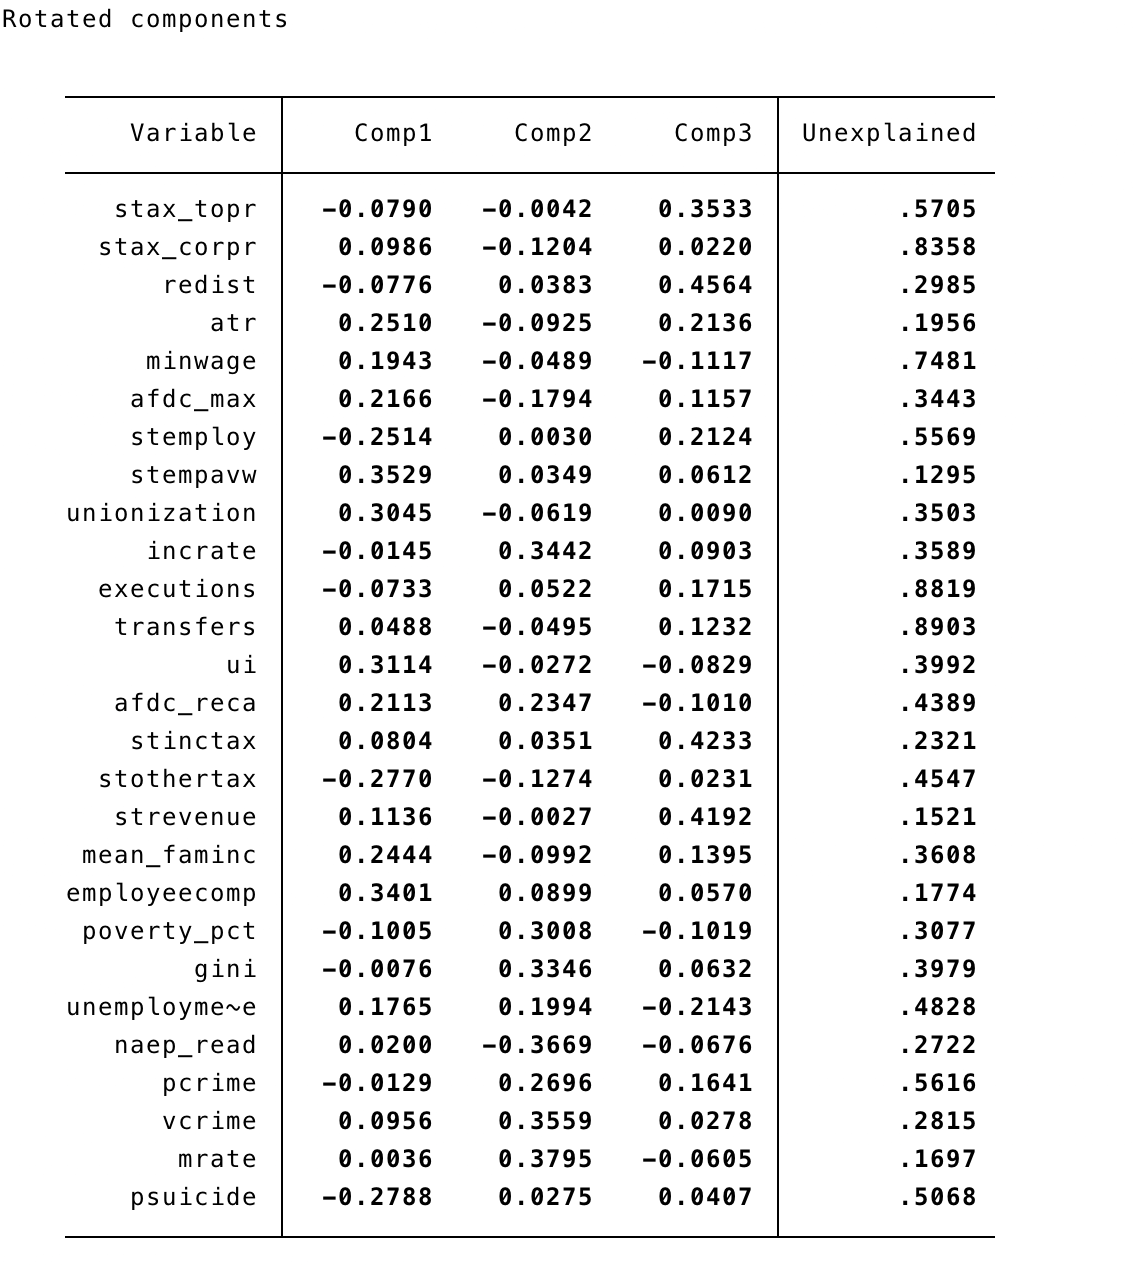
\includegraphics[width=15cm]{output/tables/pca_rotated_vars}
\\ \\
\textbf{Note:} Rotations are used to explicate simple structure and to identify clusters of correlated variables; in this case, for each component, large coefficients indicate that the factor loads on the variable more. The final column is the unexplained variance remaining after three components have been loaded.
\label{table:pca_rotated_vars}
\end{table}

\begin{table}[!hbtp]
\caption{PCA Rotated Components Variance}
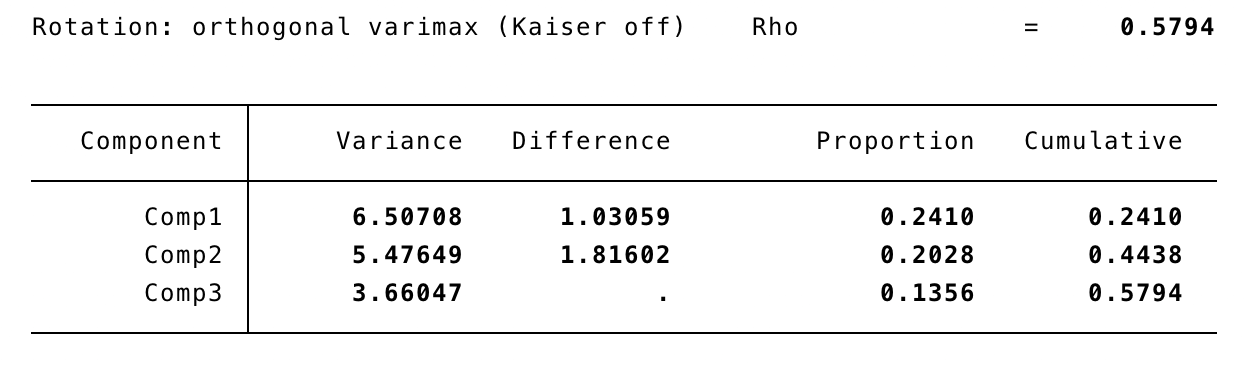
\includegraphics[width=15cm]{output/tables/pca_rotated_comp}
\\ \\
\textbf{Note:} The first column indicates the variance in the data explained by each component, while the third and fourth columns show this as a percentage of the total variance.
\label{table:pca_rotated_comp}
\end{table}

%%%%%%% REGRESSIONS %%%%%%%%

%% a %% 

\begin{table}[!hbtp]
\caption{Effect of Democratic Governor on State Policies}
\begin{center}
\begin{tabular}{lccccc}
\hline \noalign{\smallskip}Dep Var & (1) & (2) & (3) & (4) & (5)\\
\noalign{\smallskip}\hline \noalign{\smallskip}Top Income Tax Rate & \begin{scriptsize}-0.0376\end{scriptsize} & \begin{scriptsize}-0.1841\end{scriptsize} & \begin{scriptsize}-0.1937\end{scriptsize} & \begin{scriptsize}-0.1936\end{scriptsize} & \begin{scriptsize}-0.4456*\end{scriptsize}\\
 & \begin{scriptsize}(0.1651)\end{scriptsize} & \begin{scriptsize}(0.1602)\end{scriptsize} & \begin{scriptsize}(0.1531)\end{scriptsize} & \begin{scriptsize}(0.1531)\end{scriptsize} & \begin{scriptsize}(0.2343)\end{scriptsize}\\
\noalign{\smallskip}Top Corporate Tax Rate & \begin{scriptsize}0.0723\end{scriptsize} & \begin{scriptsize}-0.0644\end{scriptsize} & \begin{scriptsize}-0.0864\end{scriptsize} & \begin{scriptsize}-0.1114\end{scriptsize} & \begin{scriptsize}-0.3506**\end{scriptsize}\\
 & \begin{scriptsize}(0.1492)\end{scriptsize} & \begin{scriptsize}(0.1264)\end{scriptsize} & \begin{scriptsize}(0.1181)\end{scriptsize} & \begin{scriptsize}(0.1156)\end{scriptsize} & \begin{scriptsize}(0.1374)\end{scriptsize}\\
\noalign{\smallskip}Tax Redistribution Index & \begin{scriptsize}-0.0228\end{scriptsize} & \begin{scriptsize}-0.0172\end{scriptsize} & \begin{scriptsize}-0.0172\end{scriptsize} & \begin{scriptsize}-0.0173\end{scriptsize} & \begin{scriptsize}-0.0082\end{scriptsize}\\
 & \begin{scriptsize}(0.0143)\end{scriptsize} & \begin{scriptsize}(0.0130)\end{scriptsize} & \begin{scriptsize}(0.0131)\end{scriptsize} & \begin{scriptsize}(0.0139)\end{scriptsize} & \begin{scriptsize}(0.0175)\end{scriptsize}\\
\noalign{\smallskip}Average Income Tax Rate & \begin{scriptsize}0.0906\end{scriptsize} & \begin{scriptsize}0.1217\end{scriptsize} & \begin{scriptsize}0.1060\end{scriptsize} & \begin{scriptsize}0.1164\end{scriptsize} & \begin{scriptsize}0.2050\end{scriptsize}\\
 & \begin{scriptsize}(0.1300)\end{scriptsize} & \begin{scriptsize}(0.1196)\end{scriptsize} & \begin{scriptsize}(0.1184)\end{scriptsize} & \begin{scriptsize}(0.1265)\end{scriptsize} & \begin{scriptsize}(0.1467)\end{scriptsize}\\
\noalign{\smallskip}Log Real Minimum Wage & \begin{scriptsize}0.0092*\end{scriptsize} & \begin{scriptsize}0.0091*\end{scriptsize} & \begin{scriptsize}0.0089\end{scriptsize} & \begin{scriptsize}0.0085\end{scriptsize} & \begin{scriptsize}0.0059\end{scriptsize}\\
 & \begin{scriptsize}(0.0055)\end{scriptsize} & \begin{scriptsize}(0.0053)\end{scriptsize} & \begin{scriptsize}(0.0053)\end{scriptsize} & \begin{scriptsize}(0.0056)\end{scriptsize} & \begin{scriptsize}(0.0052)\end{scriptsize}\\
\noalign{\smallskip}Log Maximum Welfare Benefit (AFDC) & \begin{scriptsize}0.0012\end{scriptsize} & \begin{scriptsize}-0.0013\end{scriptsize} & \begin{scriptsize}0.0003\end{scriptsize} & \begin{scriptsize}0.0004\end{scriptsize} & \begin{scriptsize}-0.0106\end{scriptsize}\\
 & \begin{scriptsize}(0.0134)\end{scriptsize} & \begin{scriptsize}(0.0129)\end{scriptsize} & \begin{scriptsize}(0.0130)\end{scriptsize} & \begin{scriptsize}(0.0134)\end{scriptsize} & \begin{scriptsize}(0.0183)\end{scriptsize}\\
\noalign{\smallskip}Percent Population Gov Employees & \begin{scriptsize}-0.0202\end{scriptsize} & \begin{scriptsize}0.0055\end{scriptsize} & \begin{scriptsize}0.0065\end{scriptsize} & \begin{scriptsize}0.0060\end{scriptsize} & \begin{scriptsize}0.0081\end{scriptsize}\\
 & \begin{scriptsize}(0.0304)\end{scriptsize} & \begin{scriptsize}(0.0235)\end{scriptsize} & \begin{scriptsize}(0.0239)\end{scriptsize} & \begin{scriptsize}(0.0235)\end{scriptsize} & \begin{scriptsize}(0.0321)\end{scriptsize}\\
\noalign{\smallskip}Log Average Real Wage Gov Employees & \begin{scriptsize}-0.0033\end{scriptsize} & \begin{scriptsize}-0.0042\end{scriptsize} & \begin{scriptsize}-0.0053\end{scriptsize} & \begin{scriptsize}-0.0065\end{scriptsize} & \begin{scriptsize}-0.0048\end{scriptsize}\\
 & \begin{scriptsize}(0.0078)\end{scriptsize} & \begin{scriptsize}(0.0076)\end{scriptsize} & \begin{scriptsize}(0.0080)\end{scriptsize} & \begin{scriptsize}(0.0081)\end{scriptsize} & \begin{scriptsize}(0.0076)\end{scriptsize}\\
\noalign{\smallskip}\hline\end{tabular}\\
\end{center}

\textbf{Note:} Coefficients for the Democratic governor indicator variable listed with robust standard errors in parenthesis. Column 5 is the regression discontinuity (margin of victory $<$ 60\%). Columns 1 - 5 include state and year fixed effects \& cluster errors by state level. Columns 2 - 5 include demographic controls, columns 3 - 5 include controls for local legislature partisanship, and columns 4 - 5 include controls for state representatives in Congress. *, **, and *** indicate significance at the 10\%, 5\%, and 1\% significance levels, respectively.
\label{table:policies_a}
\end{table}

\begin{table}[!hbtp]
\caption{Effect of Democratic Governor on Intermediate Outcomes}
\begin{center}
\begin{tabular}{lccccc}
\hline \noalign{\smallskip}Dep Var & (1) & (2) & (3) & (4) & (5)\\
\noalign{\smallskip}\hline \noalign{\smallskip}Unionization Rate & \begin{scriptsize}-0.3040\end{scriptsize} & \begin{scriptsize}-0.2868\end{scriptsize} & \begin{scriptsize}-0.3248\end{scriptsize} & \begin{scriptsize}-0.3409\end{scriptsize} & \begin{scriptsize}-0.3124\end{scriptsize}\\
 & \begin{scriptsize}(0.2427)\end{scriptsize} & \begin{scriptsize}(0.2467)\end{scriptsize} & \begin{scriptsize}(0.2449)\end{scriptsize} & \begin{scriptsize}(0.2473)\end{scriptsize} & \begin{scriptsize}(0.3007)\end{scriptsize}\\
\noalign{\smallskip}Incarceration Rate & \begin{scriptsize}-9.5687\end{scriptsize} & \begin{scriptsize}-11.3970*\end{scriptsize} & \begin{scriptsize}-13.3071**\end{scriptsize} & \begin{scriptsize}-12.8029**\end{scriptsize} & \begin{scriptsize}-12.7568*\end{scriptsize}\\
 & \begin{scriptsize}(6.9422)\end{scriptsize} & \begin{scriptsize}(6.3649)\end{scriptsize} & \begin{scriptsize}(6.2159)\end{scriptsize} & \begin{scriptsize}(5.9304)\end{scriptsize} & \begin{scriptsize}(7.5291)\end{scriptsize}\\
\noalign{\smallskip}Executions per 100,000 & \begin{scriptsize}0.0040\end{scriptsize} & \begin{scriptsize}-0.0011\end{scriptsize} & \begin{scriptsize}-0.0009\end{scriptsize} & \begin{scriptsize}0.0044\end{scriptsize} & \begin{scriptsize}0.0006\end{scriptsize}\\
 & \begin{scriptsize}(0.0041)\end{scriptsize} & \begin{scriptsize}(0.0038)\end{scriptsize} & \begin{scriptsize}(0.0038)\end{scriptsize} & \begin{scriptsize}(0.0036)\end{scriptsize} & \begin{scriptsize}(0.0064)\end{scriptsize}\\
\noalign{\smallskip}Log State Transfers per Capita & \begin{scriptsize}-0.0195\end{scriptsize} & \begin{scriptsize}-0.0052\end{scriptsize} & \begin{scriptsize}-0.0071\end{scriptsize} & \begin{scriptsize}-0.0028\end{scriptsize} & \begin{scriptsize}0.0127\end{scriptsize}\\
 & \begin{scriptsize}(0.0283)\end{scriptsize} & \begin{scriptsize}(0.0268)\end{scriptsize} & \begin{scriptsize}(0.0274)\end{scriptsize} & \begin{scriptsize}(0.0276)\end{scriptsize} & \begin{scriptsize}(0.0302)\end{scriptsize}\\
\noalign{\smallskip}Log State UI Payments per Capita & \begin{scriptsize}-0.0032\end{scriptsize} & \begin{scriptsize}0.0074\end{scriptsize} & \begin{scriptsize}0.0082\end{scriptsize} & \begin{scriptsize}0.0069\end{scriptsize} & \begin{scriptsize}-0.0168\end{scriptsize}\\
 & \begin{scriptsize}(0.0244)\end{scriptsize} & \begin{scriptsize}(0.0244)\end{scriptsize} & \begin{scriptsize}(0.0242)\end{scriptsize} & \begin{scriptsize}(0.0244)\end{scriptsize} & \begin{scriptsize}(0.0310)\end{scriptsize}\\
\noalign{\smallskip}Percent Population on Welfare & \begin{scriptsize}0.1412\end{scriptsize} & \begin{scriptsize}0.1433\end{scriptsize} & \begin{scriptsize}0.1607*\end{scriptsize} & \begin{scriptsize}0.1618*\end{scriptsize} & \begin{scriptsize}0.0716\end{scriptsize}\\
 & \begin{scriptsize}(0.1003)\end{scriptsize} & \begin{scriptsize}(0.0900)\end{scriptsize} & \begin{scriptsize}(0.0927)\end{scriptsize} & \begin{scriptsize}(0.0963)\end{scriptsize} & \begin{scriptsize}(0.1104)\end{scriptsize}\\
\noalign{\smallskip}Log Real State Income Tax Receipt per Capita & \begin{scriptsize}-0.0665\end{scriptsize} & \begin{scriptsize}-0.0403\end{scriptsize} & \begin{scriptsize}-0.0305\end{scriptsize} & \begin{scriptsize}-0.0264\end{scriptsize} & \begin{scriptsize}-0.0992\end{scriptsize}\\
 & \begin{scriptsize}(0.0415)\end{scriptsize} & \begin{scriptsize}(0.0380)\end{scriptsize} & \begin{scriptsize}(0.0369)\end{scriptsize} & \begin{scriptsize}(0.0373)\end{scriptsize} & \begin{scriptsize}(0.0612)\end{scriptsize}\\
\noalign{\smallskip}Log Real Other Income Tax Receipt per Capita & \begin{scriptsize}0.0068\end{scriptsize} & \begin{scriptsize}0.0201\end{scriptsize} & \begin{scriptsize}0.0227\end{scriptsize} & \begin{scriptsize}0.0201\end{scriptsize} & \begin{scriptsize}0.0430\end{scriptsize}\\
 & \begin{scriptsize}(0.0295)\end{scriptsize} & \begin{scriptsize}(0.0279)\end{scriptsize} & \begin{scriptsize}(0.0278)\end{scriptsize} & \begin{scriptsize}(0.0278)\end{scriptsize} & \begin{scriptsize}(0.0394)\end{scriptsize}\\
\noalign{\smallskip}Log Real Non-Tax Revenue per Capita & \begin{scriptsize}0.0042\end{scriptsize} & \begin{scriptsize}0.0161\end{scriptsize} & \begin{scriptsize}0.0155\end{scriptsize} & \begin{scriptsize}0.0186\end{scriptsize} & \begin{scriptsize}0.0119\end{scriptsize}\\
 & \begin{scriptsize}(0.0359)\end{scriptsize} & \begin{scriptsize}(0.0346)\end{scriptsize} & \begin{scriptsize}(0.0358)\end{scriptsize} & \begin{scriptsize}(0.0338)\end{scriptsize} & \begin{scriptsize}(0.0329)\end{scriptsize}\\
\noalign{\smallskip}Log Real State Revenue per Capita & \begin{scriptsize}-0.0365\end{scriptsize} & \begin{scriptsize}-0.0235\end{scriptsize} & \begin{scriptsize}-0.0216\end{scriptsize} & \begin{scriptsize}-0.0192\end{scriptsize} & \begin{scriptsize}-0.0726*\end{scriptsize}\\
 & \begin{scriptsize}(0.0365)\end{scriptsize} & \begin{scriptsize}(0.0332)\end{scriptsize} & \begin{scriptsize}(0.0323)\end{scriptsize} & \begin{scriptsize}(0.0315)\end{scriptsize} & \begin{scriptsize}(0.0385)\end{scriptsize}\\
\noalign{\smallskip}\hline\end{tabular}\\
\end{center}

\textbf{Note:} Coefficients for the Democratic governor indicator variable listed with robust standard errors in parenthesis. Column 5 is the regression discontinuity (margin of victory $<$ 60\%). Columns 1 - 5 include state and year fixed effects \& cluster errors by state level. Columns 2 - 5 include demographic controls, columns 3 - 5 include controls for local legislature partisanship, and columns 4 - 5 include controls for state representatives in Congress. *, **, and *** indicate significance at the 10\%, 5\%, and 1\% significance levels, respectively.
\label{table:outcome_a}
\end{table}

\begin{table}[!hbtp]
\caption{Effect of Democratic Governor on Welfare Outcomes - Income}
\begin{center}
\begin{tabular}{lccccc}
\hline \noalign{\smallskip}Dep Var & (1) & (2) & (3) & (4) & (5)\\
\noalign{\smallskip}\hline \noalign{\smallskip}Log Real Mean Family Pre-Tax Income & \begin{scriptsize}-0.0003\end{scriptsize} & \begin{scriptsize}0.0005\end{scriptsize} & \begin{scriptsize}-0.0003\end{scriptsize} & \begin{scriptsize}-0.0001\end{scriptsize} & \begin{scriptsize}0.0082\end{scriptsize}\\
 & \begin{scriptsize}(0.0071)\end{scriptsize} & \begin{scriptsize}(0.0067)\end{scriptsize} & \begin{scriptsize}(0.0066)\end{scriptsize} & \begin{scriptsize}(0.0068)\end{scriptsize} & \begin{scriptsize}(0.0094)\end{scriptsize}\\
\noalign{\smallskip}Log Real Mean Family Post-Tax Income & \begin{scriptsize}0.0066\end{scriptsize} & \begin{scriptsize}0.0070\end{scriptsize} & \begin{scriptsize}0.0065\end{scriptsize} & \begin{scriptsize}0.0063\end{scriptsize} & \begin{scriptsize}0.0098\end{scriptsize}\\
 & \begin{scriptsize}(0.0059)\end{scriptsize} & \begin{scriptsize}(0.0052)\end{scriptsize} & \begin{scriptsize}(0.0052)\end{scriptsize} & \begin{scriptsize}(0.0054)\end{scriptsize} & \begin{scriptsize}(0.0085)\end{scriptsize}\\
\noalign{\smallskip}Log Real Median Family Pre-Tax Income & \begin{scriptsize}0.0007\end{scriptsize} & \begin{scriptsize}0.0025\end{scriptsize} & \begin{scriptsize}0.0020\end{scriptsize} & \begin{scriptsize}0.0023\end{scriptsize} & \begin{scriptsize}0.0098\end{scriptsize}\\
 & \begin{scriptsize}(0.0077)\end{scriptsize} & \begin{scriptsize}(0.0071)\end{scriptsize} & \begin{scriptsize}(0.0070)\end{scriptsize} & \begin{scriptsize}(0.0073)\end{scriptsize} & \begin{scriptsize}(0.0105)\end{scriptsize}\\
\noalign{\smallskip}Log Real Median Family Post-Tax Income & \begin{scriptsize}0.0105\end{scriptsize} & \begin{scriptsize}0.0120*\end{scriptsize} & \begin{scriptsize}0.0120*\end{scriptsize} & \begin{scriptsize}0.0123*\end{scriptsize} & \begin{scriptsize}0.0145\end{scriptsize}\\
 & \begin{scriptsize}(0.0068)\end{scriptsize} & \begin{scriptsize}(0.0061)\end{scriptsize} & \begin{scriptsize}(0.0060)\end{scriptsize} & \begin{scriptsize}(0.0064)\end{scriptsize} & \begin{scriptsize}(0.0095)\end{scriptsize}\\
\noalign{\smallskip}Log Mean Real Wage & \begin{scriptsize}-0.0067\end{scriptsize} & \begin{scriptsize}-0.0063\end{scriptsize} & \begin{scriptsize}-0.0076\end{scriptsize} & \begin{scriptsize}-0.0086\end{scriptsize} & \begin{scriptsize}-0.0069\end{scriptsize}\\
 & \begin{scriptsize}(0.0126)\end{scriptsize} & \begin{scriptsize}(0.0115)\end{scriptsize} & \begin{scriptsize}(0.0117)\end{scriptsize} & \begin{scriptsize}(0.0125)\end{scriptsize} & \begin{scriptsize}(0.0114)\end{scriptsize}\\
\noalign{\smallskip}Percent Population Poverty & \begin{scriptsize}0.0889\end{scriptsize} & \begin{scriptsize}-0.0849\end{scriptsize} & \begin{scriptsize}-0.0657\end{scriptsize} & \begin{scriptsize}-0.0459\end{scriptsize} & \begin{scriptsize}-0.5817\end{scriptsize}\\
 & \begin{scriptsize}(0.6625)\end{scriptsize} & \begin{scriptsize}(0.5818)\end{scriptsize} & \begin{scriptsize}(0.5821)\end{scriptsize} & \begin{scriptsize}(0.5797)\end{scriptsize} & \begin{scriptsize}(0.7129)\end{scriptsize}\\
\noalign{\smallskip}Pre-Tax Gini & \begin{scriptsize}0.0850\end{scriptsize} & \begin{scriptsize}0.0112\end{scriptsize} & \begin{scriptsize}0.0008\end{scriptsize} & \begin{scriptsize}-0.0119\end{scriptsize} & \begin{scriptsize}-0.1166\end{scriptsize}\\
 & \begin{scriptsize}(0.1442)\end{scriptsize} & \begin{scriptsize}(0.1336)\end{scriptsize} & \begin{scriptsize}(0.1377)\end{scriptsize} & \begin{scriptsize}(0.1362)\end{scriptsize} & \begin{scriptsize}(0.1823)\end{scriptsize}\\
\noalign{\smallskip}Post-Tax Gini & \begin{scriptsize}-0.2258\end{scriptsize} & \begin{scriptsize}-0.2954*\end{scriptsize} & \begin{scriptsize}-0.3011*\end{scriptsize} & \begin{scriptsize}-0.3262*\end{scriptsize} & \begin{scriptsize}-0.3736*\end{scriptsize}\\
 & \begin{scriptsize}(0.1765)\end{scriptsize} & \begin{scriptsize}(0.1622)\end{scriptsize} & \begin{scriptsize}(0.1672)\end{scriptsize} & \begin{scriptsize}(0.1787)\end{scriptsize} & \begin{scriptsize}(0.1946)\end{scriptsize}\\
\noalign{\smallskip}\hline\end{tabular}\\
\end{center}

\textbf{Note:} Coefficients for the Democratic governor indicator variable listed with robust standard errors in parenthesis. Column 5 is the regression discontinuity (margin of victory $<$ 60\%). Columns 1 - 5 include state and year fixed effects \& cluster errors by state level. Columns 2 - 5 include demographic controls, columns 3 - 5 include controls for local legislature partisanship, and columns 4 - 5 include controls for state representatives in Congress. *, **, and *** indicate significance at the 10\%, 5\%, and 1\% significance levels, respectively.
\label{table:welfare1_a}
\end{table}

\begin{table}[!hbtp]
\caption{Effect of Democratic Governor on Welfare Outcomes - Work and Crime}
\begin{center}
\begin{tabular}{lccccc}
\hline \noalign{\smallskip}Dep Var & (1) & (2) & (3) & (4) & (5)\\
\noalign{\smallskip}\hline \noalign{\smallskip}Unemployment Rate & \begin{scriptsize}-0.1831\end{scriptsize} & \begin{scriptsize}-0.1892\end{scriptsize} & \begin{scriptsize}-0.1806\end{scriptsize} & \begin{scriptsize}-0.1895\end{scriptsize} & \begin{scriptsize}-0.3179*\end{scriptsize}\\
 & \begin{scriptsize}(0.1128)\end{scriptsize} & \begin{scriptsize}(0.1198)\end{scriptsize} & \begin{scriptsize}(0.1247)\end{scriptsize} & \begin{scriptsize}(0.1301)\end{scriptsize} & \begin{scriptsize}(0.1615)\end{scriptsize}\\
\noalign{\smallskip}Average NAEP 4th Grade Score & \begin{scriptsize}-0.2409\end{scriptsize} & \begin{scriptsize}0.2875\end{scriptsize} & \begin{scriptsize}0.2937\end{scriptsize} & \begin{scriptsize}0.2431\end{scriptsize} & \begin{scriptsize}0.4398\end{scriptsize}\\
 & \begin{scriptsize}(0.4409)\end{scriptsize} & \begin{scriptsize}(0.4417)\end{scriptsize} & \begin{scriptsize}(0.4371)\end{scriptsize} & \begin{scriptsize}(0.4339)\end{scriptsize} & \begin{scriptsize}(0.5760)\end{scriptsize}\\
\noalign{\smallskip}Property Crimes per 100,000 & \begin{scriptsize}-48.6971\end{scriptsize} & \begin{scriptsize}-50.5024\end{scriptsize} & \begin{scriptsize}-48.9210\end{scriptsize} & \begin{scriptsize}-45.2274\end{scriptsize} & \begin{scriptsize}65.5612\end{scriptsize}\\
 & \begin{scriptsize}(42.6842)\end{scriptsize} & \begin{scriptsize}(39.0732)\end{scriptsize} & \begin{scriptsize}(39.2171)\end{scriptsize} & \begin{scriptsize}(38.4858)\end{scriptsize} & \begin{scriptsize}(57.5868)\end{scriptsize}\\
\noalign{\smallskip}Violent Crimes per 100,000 & \begin{scriptsize}-2.8772\end{scriptsize} & \begin{scriptsize}-6.6346\end{scriptsize} & \begin{scriptsize}-6.8461\end{scriptsize} & \begin{scriptsize}-6.3962\end{scriptsize} & \begin{scriptsize}-4.4936\end{scriptsize}\\
 & \begin{scriptsize}(10.2512)\end{scriptsize} & \begin{scriptsize}(9.7557)\end{scriptsize} & \begin{scriptsize}(9.5706)\end{scriptsize} & \begin{scriptsize}(9.3194)\end{scriptsize} & \begin{scriptsize}(10.4492)\end{scriptsize}\\
\noalign{\smallskip}Murder Rate per 100,000 & \begin{scriptsize}-0.0688\end{scriptsize} & \begin{scriptsize}-0.0956\end{scriptsize} & \begin{scriptsize}-0.0685\end{scriptsize} & \begin{scriptsize}-0.0893\end{scriptsize} & \begin{scriptsize}-0.0178\end{scriptsize}\\
 & \begin{scriptsize}(0.1436)\end{scriptsize} & \begin{scriptsize}(0.1320)\end{scriptsize} & \begin{scriptsize}(0.1283)\end{scriptsize} & \begin{scriptsize}(0.1283)\end{scriptsize} & \begin{scriptsize}(0.1454)\end{scriptsize}\\
\noalign{\smallskip}Suicide Rate per 100,000 & \begin{scriptsize}-0.2211*\end{scriptsize} & \begin{scriptsize}-0.1412\end{scriptsize} & \begin{scriptsize}-0.1215\end{scriptsize} & \begin{scriptsize}-0.1041\end{scriptsize} & \begin{scriptsize}-0.1721\end{scriptsize}\\
 & \begin{scriptsize}(0.1270)\end{scriptsize} & \begin{scriptsize}(0.1162)\end{scriptsize} & \begin{scriptsize}(0.1145)\end{scriptsize} & \begin{scriptsize}(0.1133)\end{scriptsize} & \begin{scriptsize}(0.1866)\end{scriptsize}\\
\noalign{\smallskip}\hline\end{tabular}\\
\end{center}

\textbf{Note:} Coefficients for the Democratic governor indicator variable listed with robust standard errors in parenthesis. Column 5 is the regression discontinuity (margin of victory $<$ 60\%). Columns 1 - 5 include state and year fixed effects \& cluster errors by state level. Columns 2 - 5 include demographic controls, columns 3 - 5 include controls for local legislature partisanship, and columns 4 - 5 include controls for state representatives in Congress. *, **, and *** indicate significance at the 10\%, 5\%, and 1\% significance levels, respectively.
\label{table:welfare2_a}
\end{table}

\begin{table}[!hbtp]
\caption{Effect of Democratic Governor on Abortion}
\estwide{output/tables/abortion_a}{5}{c}
\textbf{Note:} Coefficients for the Democratic governor indicator variable listed with robust standard errors in parenthesis. Column 5 is the regression discontinuity (margin of victory $<$ 60\%). Columns 1 - 5 include state and year fixed effects \& cluster errors by state level. Columns 2 - 5 include demographic controls, columns 3 - 5 include controls for local legislature partisanship, and columns 4 - 5 include controls for state representatives in Congress. *, **, and *** indicate significance at the 10\%, 5\%, and 1\% significance levels, respectively.
\label{table:abortion_a}
\end{table}

\begin{table}[!hbtp]
\caption{Effect of Democratic Governor on Indices}
\begin{center}
\begin{tabular}{lccccc}
\hline \noalign{\smallskip}Dep Var & (1) & (2) & (3) & (4) & (5)\\
\noalign{\smallskip}\hline \noalign{\smallskip}Social Safety Index & \begin{scriptsize}-0.0371\end{scriptsize} & \begin{scriptsize}-0.0030\end{scriptsize} & \begin{scriptsize}0.0022\end{scriptsize} & \begin{scriptsize}-0.0010\end{scriptsize} & \begin{scriptsize}-0.0210\end{scriptsize}\\
 & \begin{scriptsize}(0.0937)\end{scriptsize} & \begin{scriptsize}(0.0995)\end{scriptsize} & \begin{scriptsize}(0.0932)\end{scriptsize} & \begin{scriptsize}(0.0942)\end{scriptsize} & \begin{scriptsize}(0.1469)\end{scriptsize}\\
\noalign{\smallskip}Crime/Inequality Index & \begin{scriptsize}0.0192\end{scriptsize} & \begin{scriptsize}0.0238\end{scriptsize} & \begin{scriptsize}0.0199\end{scriptsize} & \begin{scriptsize}0.0096\end{scriptsize} & \begin{scriptsize}-0.0306\end{scriptsize}\\
 & \begin{scriptsize}(0.0810)\end{scriptsize} & \begin{scriptsize}(0.0791)\end{scriptsize} & \begin{scriptsize}(0.0753)\end{scriptsize} & \begin{scriptsize}(0.0736)\end{scriptsize} & \begin{scriptsize}(0.0863)\end{scriptsize}\\
\noalign{\smallskip}Gov. Size Index & \begin{scriptsize}-0.0091\end{scriptsize} & \begin{scriptsize}0.0161\end{scriptsize} & \begin{scriptsize}0.0168\end{scriptsize} & \begin{scriptsize}0.0218\end{scriptsize} & \begin{scriptsize}-0.0163\end{scriptsize}\\
 & \begin{scriptsize}(0.0988)\end{scriptsize} & \begin{scriptsize}(0.0899)\end{scriptsize} & \begin{scriptsize}(0.0895)\end{scriptsize} & \begin{scriptsize}(0.0894)\end{scriptsize} & \begin{scriptsize}(0.1257)\end{scriptsize}\\
\noalign{\smallskip}\hline\end{tabular}\\
\end{center}

\textbf{Note:} Coefficients for the Democratic governor indicator variable listed with robust standard errors in parenthesis. Column 5 is the regression discontinuity (margin of victory $<$ 60\%). Columns 1 - 5 include state and year fixed effects \& cluster errors by state level. Columns 2 - 5 include demographic controls, columns 3 - 5 include controls for local legislature partisanship, and columns 4 - 5 include controls for state representatives in Congress. *, **, and *** indicate significance at the 10\%, 5\%, and 1\% significance levels, respectively.
\label{table:index_a}
\end{table}


%% b %%

\begin{table}[!hbtp]
\caption{Effect of Democratic Governor on State Policies - Omit First Year}
\begin{center}
\begin{tabular}{lccccc}
\hline \noalign{\smallskip}Dep Var & (1) & (2) & (3) & (4) & (5)\\
\noalign{\smallskip}\hline \noalign{\smallskip}Top Income Tax Rate & \begin{scriptsize}-0.0400\end{scriptsize} & \begin{scriptsize}-0.1645\end{scriptsize} & \begin{scriptsize}-0.1628\end{scriptsize} & \begin{scriptsize}-0.1625\end{scriptsize} & \begin{scriptsize}-0.3867\end{scriptsize}\\
 & \begin{scriptsize}(0.1759)\end{scriptsize} & \begin{scriptsize}(0.1683)\end{scriptsize} & \begin{scriptsize}(0.1602)\end{scriptsize} & \begin{scriptsize}(0.1601)\end{scriptsize} & \begin{scriptsize}(0.2485)\end{scriptsize}\\
\noalign{\smallskip}Top Corporate Tax Rate & \begin{scriptsize}0.0605\end{scriptsize} & \begin{scriptsize}-0.0723\end{scriptsize} & \begin{scriptsize}-0.0818\end{scriptsize} & \begin{scriptsize}-0.1018\end{scriptsize} & \begin{scriptsize}-0.3499**\end{scriptsize}\\
 & \begin{scriptsize}(0.1530)\end{scriptsize} & \begin{scriptsize}(0.1286)\end{scriptsize} & \begin{scriptsize}(0.1211)\end{scriptsize} & \begin{scriptsize}(0.1199)\end{scriptsize} & \begin{scriptsize}(0.1408)\end{scriptsize}\\
\noalign{\smallskip}Tax Redistribution Index & \begin{scriptsize}-0.0271*\end{scriptsize} & \begin{scriptsize}-0.0206\end{scriptsize} & \begin{scriptsize}-0.0195\end{scriptsize} & \begin{scriptsize}-0.0197\end{scriptsize} & \begin{scriptsize}-0.0131\end{scriptsize}\\
 & \begin{scriptsize}(0.0160)\end{scriptsize} & \begin{scriptsize}(0.0149)\end{scriptsize} & \begin{scriptsize}(0.0147)\end{scriptsize} & \begin{scriptsize}(0.0155)\end{scriptsize} & \begin{scriptsize}(0.0199)\end{scriptsize}\\
\noalign{\smallskip}Average Income Tax Rate & \begin{scriptsize}0.0721\end{scriptsize} & \begin{scriptsize}0.1036\end{scriptsize} & \begin{scriptsize}0.0937\end{scriptsize} & \begin{scriptsize}0.0959\end{scriptsize} & \begin{scriptsize}0.1650\end{scriptsize}\\
 & \begin{scriptsize}(0.1425)\end{scriptsize} & \begin{scriptsize}(0.1323)\end{scriptsize} & \begin{scriptsize}(0.1305)\end{scriptsize} & \begin{scriptsize}(0.1379)\end{scriptsize} & \begin{scriptsize}(0.1663)\end{scriptsize}\\
\noalign{\smallskip}Log Real Minimum Wage & \begin{scriptsize}0.0109*\end{scriptsize} & \begin{scriptsize}0.0104*\end{scriptsize} & \begin{scriptsize}0.0106*\end{scriptsize} & \begin{scriptsize}0.0105\end{scriptsize} & \begin{scriptsize}0.0104\end{scriptsize}\\
 & \begin{scriptsize}(0.0061)\end{scriptsize} & \begin{scriptsize}(0.0059)\end{scriptsize} & \begin{scriptsize}(0.0060)\end{scriptsize} & \begin{scriptsize}(0.0063)\end{scriptsize} & \begin{scriptsize}(0.0073)\end{scriptsize}\\
\noalign{\smallskip}Log Maximum Welfare Benefit (AFDC) & \begin{scriptsize}0.0022\end{scriptsize} & \begin{scriptsize}-0.0001\end{scriptsize} & \begin{scriptsize}0.0022\end{scriptsize} & \begin{scriptsize}0.0020\end{scriptsize} & \begin{scriptsize}-0.0110\end{scriptsize}\\
 & \begin{scriptsize}(0.0132)\end{scriptsize} & \begin{scriptsize}(0.0129)\end{scriptsize} & \begin{scriptsize}(0.0128)\end{scriptsize} & \begin{scriptsize}(0.0132)\end{scriptsize} & \begin{scriptsize}(0.0188)\end{scriptsize}\\
\noalign{\smallskip}Percent Population Gov Employees & \begin{scriptsize}-0.0319\end{scriptsize} & \begin{scriptsize}0.0047\end{scriptsize} & \begin{scriptsize}0.0072\end{scriptsize} & \begin{scriptsize}0.0061\end{scriptsize} & \begin{scriptsize}0.0104\end{scriptsize}\\
 & \begin{scriptsize}(0.0320)\end{scriptsize} & \begin{scriptsize}(0.0252)\end{scriptsize} & \begin{scriptsize}(0.0256)\end{scriptsize} & \begin{scriptsize}(0.0248)\end{scriptsize} & \begin{scriptsize}(0.0326)\end{scriptsize}\\
\noalign{\smallskip}Log Average Real Wage Gov Employees & \begin{scriptsize}-0.0040\end{scriptsize} & \begin{scriptsize}-0.0057\end{scriptsize} & \begin{scriptsize}-0.0072\end{scriptsize} & \begin{scriptsize}-0.0083\end{scriptsize} & \begin{scriptsize}-0.0061\end{scriptsize}\\
 & \begin{scriptsize}(0.0086)\end{scriptsize} & \begin{scriptsize}(0.0085)\end{scriptsize} & \begin{scriptsize}(0.0089)\end{scriptsize} & \begin{scriptsize}(0.0091)\end{scriptsize} & \begin{scriptsize}(0.0080)\end{scriptsize}\\
\noalign{\smallskip}\hline\end{tabular}\\
\end{center}

\textbf{Note:} The first year of each governor's term is dropped. Coefficients for the Democratic governor indicator variable listed with robust standard errors in parenthesis. Column 5 is the regression discontinuity (margin of victory $<$ 60\%). Columns 1 - 5 include state and year fixed effects \& cluster errors by state level. Columns 2 - 5 include demographic controls, columns 3 - 5 include controls for local legislature partisanship, and columns 4 - 5 include controls for state representatives in Congress. *, **, and *** indicate significance at the 10\%, 5\%, and 1\% significance levels, respectively.
\label{table:policies_b}
\end{table}

\begin{table}[!hbtp]
\caption{Effect of Democratic Governor on Intermediate Outcomes - Omit First Year}
\begin{center}
\begin{tabular}{lccccc}
\hline \noalign{\smallskip}Dep Var & (1) & (2) & (3) & (4) & (5)\\
\noalign{\smallskip}\hline \noalign{\smallskip}Unionization Rate & \begin{scriptsize}-0.3078\end{scriptsize} & \begin{scriptsize}-0.2765\end{scriptsize} & \begin{scriptsize}-0.3300\end{scriptsize} & \begin{scriptsize}-0.3480\end{scriptsize} & \begin{scriptsize}-0.2774\end{scriptsize}\\
 & \begin{scriptsize}(0.2351)\end{scriptsize} & \begin{scriptsize}(0.2390)\end{scriptsize} & \begin{scriptsize}(0.2399)\end{scriptsize} & \begin{scriptsize}(0.2411)\end{scriptsize} & \begin{scriptsize}(0.2946)\end{scriptsize}\\
\noalign{\smallskip}Incarceration Rate & \begin{scriptsize}-8.4465\end{scriptsize} & \begin{scriptsize}-10.0978\end{scriptsize} & \begin{scriptsize}-12.7136**\end{scriptsize} & \begin{scriptsize}-12.3466**\end{scriptsize} & \begin{scriptsize}-11.1447\end{scriptsize}\\
 & \begin{scriptsize}(7.0708)\end{scriptsize} & \begin{scriptsize}(6.5177)\end{scriptsize} & \begin{scriptsize}(6.1303)\end{scriptsize} & \begin{scriptsize}(5.9103)\end{scriptsize} & \begin{scriptsize}(7.9616)\end{scriptsize}\\
\noalign{\smallskip}Executions per 100,000 & \begin{scriptsize}0.0013\end{scriptsize} & \begin{scriptsize}-0.0033\end{scriptsize} & \begin{scriptsize}-0.0031\end{scriptsize} & \begin{scriptsize}0.0031\end{scriptsize} & \begin{scriptsize}0.0020\end{scriptsize}\\
 & \begin{scriptsize}(0.0043)\end{scriptsize} & \begin{scriptsize}(0.0044)\end{scriptsize} & \begin{scriptsize}(0.0042)\end{scriptsize} & \begin{scriptsize}(0.0044)\end{scriptsize} & \begin{scriptsize}(0.0070)\end{scriptsize}\\
\noalign{\smallskip}Log State Transfers per Capita & \begin{scriptsize}-0.0214\end{scriptsize} & \begin{scriptsize}-0.0068\end{scriptsize} & \begin{scriptsize}-0.0100\end{scriptsize} & \begin{scriptsize}-0.0060\end{scriptsize} & \begin{scriptsize}0.0165\end{scriptsize}\\
 & \begin{scriptsize}(0.0301)\end{scriptsize} & \begin{scriptsize}(0.0284)\end{scriptsize} & \begin{scriptsize}(0.0288)\end{scriptsize} & \begin{scriptsize}(0.0289)\end{scriptsize} & \begin{scriptsize}(0.0315)\end{scriptsize}\\
\noalign{\smallskip}Log State UI Payments per Capita & \begin{scriptsize}0.0037\end{scriptsize} & \begin{scriptsize}0.0152\end{scriptsize} & \begin{scriptsize}0.0155\end{scriptsize} & \begin{scriptsize}0.0135\end{scriptsize} & \begin{scriptsize}-0.0005\end{scriptsize}\\
 & \begin{scriptsize}(0.0246)\end{scriptsize} & \begin{scriptsize}(0.0247)\end{scriptsize} & \begin{scriptsize}(0.0243)\end{scriptsize} & \begin{scriptsize}(0.0242)\end{scriptsize} & \begin{scriptsize}(0.0336)\end{scriptsize}\\
\noalign{\smallskip}Percent Population on Welfare & \begin{scriptsize}0.1539\end{scriptsize} & \begin{scriptsize}0.1582\end{scriptsize} & \begin{scriptsize}0.1867*\end{scriptsize} & \begin{scriptsize}0.1865*\end{scriptsize} & \begin{scriptsize}0.1058\end{scriptsize}\\
 & \begin{scriptsize}(0.1054)\end{scriptsize} & \begin{scriptsize}(0.0949)\end{scriptsize} & \begin{scriptsize}(0.0998)\end{scriptsize} & \begin{scriptsize}(0.1031)\end{scriptsize} & \begin{scriptsize}(0.1199)\end{scriptsize}\\
\noalign{\smallskip}Log Real State Income Tax Receipt per Capita & \begin{scriptsize}-0.0528\end{scriptsize} & \begin{scriptsize}-0.0253\end{scriptsize} & \begin{scriptsize}-0.0111\end{scriptsize} & \begin{scriptsize}-0.0082\end{scriptsize} & \begin{scriptsize}-0.0899\end{scriptsize}\\
 & \begin{scriptsize}(0.0414)\end{scriptsize} & \begin{scriptsize}(0.0401)\end{scriptsize} & \begin{scriptsize}(0.0409)\end{scriptsize} & \begin{scriptsize}(0.0412)\end{scriptsize} & \begin{scriptsize}(0.0651)\end{scriptsize}\\
\noalign{\smallskip}Log Real Other Income Tax Receipt per Capita & \begin{scriptsize}0.0095\end{scriptsize} & \begin{scriptsize}0.0271\end{scriptsize} & \begin{scriptsize}0.0286\end{scriptsize} & \begin{scriptsize}0.0275\end{scriptsize} & \begin{scriptsize}0.0620\end{scriptsize}\\
 & \begin{scriptsize}(0.0313)\end{scriptsize} & \begin{scriptsize}(0.0299)\end{scriptsize} & \begin{scriptsize}(0.0293)\end{scriptsize} & \begin{scriptsize}(0.0290)\end{scriptsize} & \begin{scriptsize}(0.0380)\end{scriptsize}\\
\noalign{\smallskip}Log Real Non-Tax Revenue per Capita & \begin{scriptsize}0.0078\end{scriptsize} & \begin{scriptsize}0.0227\end{scriptsize} & \begin{scriptsize}0.0224\end{scriptsize} & \begin{scriptsize}0.0231\end{scriptsize} & \begin{scriptsize}0.0171\end{scriptsize}\\
 & \begin{scriptsize}(0.0358)\end{scriptsize} & \begin{scriptsize}(0.0344)\end{scriptsize} & \begin{scriptsize}(0.0354)\end{scriptsize} & \begin{scriptsize}(0.0340)\end{scriptsize} & \begin{scriptsize}(0.0333)\end{scriptsize}\\
\noalign{\smallskip}Log Real State Revenue per Capita & \begin{scriptsize}-0.0362\end{scriptsize} & \begin{scriptsize}-0.0211\end{scriptsize} & \begin{scriptsize}-0.0158\end{scriptsize} & \begin{scriptsize}-0.0137\end{scriptsize} & \begin{scriptsize}-0.0706*\end{scriptsize}\\
 & \begin{scriptsize}(0.0356)\end{scriptsize} & \begin{scriptsize}(0.0338)\end{scriptsize} & \begin{scriptsize}(0.0323)\end{scriptsize} & \begin{scriptsize}(0.0317)\end{scriptsize} & \begin{scriptsize}(0.0395)\end{scriptsize}\\
\noalign{\smallskip}\hline\end{tabular}\\
\end{center}

\textbf{Note:} The first year of each governor's term is dropped. Coefficients for the Democratic governor indicator variable listed with robust standard errors in parenthesis. Column 5 is the regression discontinuity (margin of victory $<$ 60\%). Columns 1 - 5 include state and year fixed effects \& cluster errors by state level. Columns 2 - 5 include demographic controls, columns 3 - 5 include controls for local legislature partisanship, and columns 4 - 5 include controls for state representatives in Congress. *, **, and *** indicate significance at the 10\%, 5\%, and 1\% significance levels, respectively.
\label{table:outcome_b}
\end{table}

\begin{table}[!hbtp]
\caption{Effect of Democratic Governor on Welfare Outcomes - Income - Omit First Year}
\begin{center}
\begin{tabular}{lccccc}
\hline \noalign{\smallskip}Dep Var & (1) & (2) & (3) & (4) & (5)\\
\noalign{\smallskip}\hline \noalign{\smallskip}Log Real Mean Family Pre-Tax Income & \begin{scriptsize}-0.0027\end{scriptsize} & \begin{scriptsize}-0.0018\end{scriptsize} & \begin{scriptsize}-0.0028\end{scriptsize} & \begin{scriptsize}-0.0030\end{scriptsize} & \begin{scriptsize}0.0042\end{scriptsize}\\
 & \begin{scriptsize}(0.0075)\end{scriptsize} & \begin{scriptsize}(0.0073)\end{scriptsize} & \begin{scriptsize}(0.0072)\end{scriptsize} & \begin{scriptsize}(0.0075)\end{scriptsize} & \begin{scriptsize}(0.0103)\end{scriptsize}\\
\noalign{\smallskip}Log Real Mean Family Post-Tax Income & \begin{scriptsize}0.0052\end{scriptsize} & \begin{scriptsize}0.0055\end{scriptsize} & \begin{scriptsize}0.0045\end{scriptsize} & \begin{scriptsize}0.0039\end{scriptsize} & \begin{scriptsize}0.0080\end{scriptsize}\\
 & \begin{scriptsize}(0.0061)\end{scriptsize} & \begin{scriptsize}(0.0053)\end{scriptsize} & \begin{scriptsize}(0.0053)\end{scriptsize} & \begin{scriptsize}(0.0054)\end{scriptsize} & \begin{scriptsize}(0.0091)\end{scriptsize}\\
\noalign{\smallskip}Log Real Median Family Pre-Tax Income & \begin{scriptsize}-0.0008\end{scriptsize} & \begin{scriptsize}0.0014\end{scriptsize} & \begin{scriptsize}0.0006\end{scriptsize} & \begin{scriptsize}0.0008\end{scriptsize} & \begin{scriptsize}0.0042\end{scriptsize}\\
 & \begin{scriptsize}(0.0078)\end{scriptsize} & \begin{scriptsize}(0.0074)\end{scriptsize} & \begin{scriptsize}(0.0073)\end{scriptsize} & \begin{scriptsize}(0.0076)\end{scriptsize} & \begin{scriptsize}(0.0108)\end{scriptsize}\\
\noalign{\smallskip}Log Real Median Family Post-Tax Income & \begin{scriptsize}0.0096\end{scriptsize} & \begin{scriptsize}0.0109*\end{scriptsize} & \begin{scriptsize}0.0107*\end{scriptsize} & \begin{scriptsize}0.0109*\end{scriptsize} & \begin{scriptsize}0.0115\end{scriptsize}\\
 & \begin{scriptsize}(0.0069)\end{scriptsize} & \begin{scriptsize}(0.0062)\end{scriptsize} & \begin{scriptsize}(0.0062)\end{scriptsize} & \begin{scriptsize}(0.0065)\end{scriptsize} & \begin{scriptsize}(0.0102)\end{scriptsize}\\
\noalign{\smallskip}Log Mean Real Wage & \begin{scriptsize}-0.0077\end{scriptsize} & \begin{scriptsize}-0.0077\end{scriptsize} & \begin{scriptsize}-0.0089\end{scriptsize} & \begin{scriptsize}-0.0098\end{scriptsize} & \begin{scriptsize}-0.0079\end{scriptsize}\\
 & \begin{scriptsize}(0.0148)\end{scriptsize} & \begin{scriptsize}(0.0135)\end{scriptsize} & \begin{scriptsize}(0.0134)\end{scriptsize} & \begin{scriptsize}(0.0143)\end{scriptsize} & \begin{scriptsize}(0.0130)\end{scriptsize}\\
\noalign{\smallskip}Percent Population Poverty & \begin{scriptsize}0.0264\end{scriptsize} & \begin{scriptsize}-0.1310\end{scriptsize} & \begin{scriptsize}-0.1071\end{scriptsize} & \begin{scriptsize}-0.1006\end{scriptsize} & \begin{scriptsize}-0.6038\end{scriptsize}\\
 & \begin{scriptsize}(0.6473)\end{scriptsize} & \begin{scriptsize}(0.5718)\end{scriptsize} & \begin{scriptsize}(0.5730)\end{scriptsize} & \begin{scriptsize}(0.5667)\end{scriptsize} & \begin{scriptsize}(0.7019)\end{scriptsize}\\
\noalign{\smallskip}Pre-Tax Gini & \begin{scriptsize}0.0054\end{scriptsize} & \begin{scriptsize}-0.0646\end{scriptsize} & \begin{scriptsize}-0.0756\end{scriptsize} & \begin{scriptsize}-0.0995\end{scriptsize} & \begin{scriptsize}-0.0947\end{scriptsize}\\
 & \begin{scriptsize}(0.1563)\end{scriptsize} & \begin{scriptsize}(0.1438)\end{scriptsize} & \begin{scriptsize}(0.1467)\end{scriptsize} & \begin{scriptsize}(0.1439)\end{scriptsize} & \begin{scriptsize}(0.2037)\end{scriptsize}\\
\noalign{\smallskip}Post-Tax Gini & \begin{scriptsize}-0.2158\end{scriptsize} & \begin{scriptsize}-0.2951*\end{scriptsize} & \begin{scriptsize}-0.3082*\end{scriptsize} & \begin{scriptsize}-0.3459*\end{scriptsize} & \begin{scriptsize}-0.2844\end{scriptsize}\\
 & \begin{scriptsize}(0.1765)\end{scriptsize} & \begin{scriptsize}(0.1615)\end{scriptsize} & \begin{scriptsize}(0.1666)\end{scriptsize} & \begin{scriptsize}(0.1751)\end{scriptsize} & \begin{scriptsize}(0.2152)\end{scriptsize}\\
\noalign{\smallskip}\hline\end{tabular}\\
\end{center}

\textbf{Note:} The first year of each governor's term is dropped. Coefficients for the Democratic governor indicator variable listed with robust standard errors in parenthesis. Column 5 is the regression discontinuity (margin of victory $<$ 60\%). Columns 1 - 5 include state and year fixed effects \& cluster errors by state level. Columns 2 - 5 include demographic controls, columns 3 - 5 include controls for local legislature partisanship, and columns 4 - 5 include controls for state representatives in Congress. *, **, and *** indicate significance at the 10\%, 5\%, and 1\% significance levels, respectively.
\label{table:welfare1_b}
\end{table}

\begin{table}[!hbtp]
\caption{Effect of Democratic Governor on Welfare Outcomes - Work and Crime - Omit First Year}
\begin{center}
\begin{tabular}{lccccc}
\hline \noalign{\smallskip}Dep Var & (1) & (2) & (3) & (4) & (5)\\
\noalign{\smallskip}\hline \noalign{\smallskip}Unemployment Rate & \begin{scriptsize}-0.1846\end{scriptsize} & \begin{scriptsize}-0.1760\end{scriptsize} & \begin{scriptsize}-0.1635\end{scriptsize} & \begin{scriptsize}-0.1727\end{scriptsize} & \begin{scriptsize}-0.2895*\end{scriptsize}\\
 & \begin{scriptsize}(0.1160)\end{scriptsize} & \begin{scriptsize}(0.1208)\end{scriptsize} & \begin{scriptsize}(0.1285)\end{scriptsize} & \begin{scriptsize}(0.1321)\end{scriptsize} & \begin{scriptsize}(0.1673)\end{scriptsize}\\
\noalign{\smallskip}Average NAEP 4th Grade Score & \begin{scriptsize}0.3775\end{scriptsize} & \begin{scriptsize}0.2828\end{scriptsize} & \begin{scriptsize}0.2880\end{scriptsize} & \begin{scriptsize}0.2575\end{scriptsize} & \begin{scriptsize}0.6204\end{scriptsize}\\
 & \begin{scriptsize}(0.4577)\end{scriptsize} & \begin{scriptsize}(0.4346)\end{scriptsize} & \begin{scriptsize}(0.4356)\end{scriptsize} & \begin{scriptsize}(0.4342)\end{scriptsize} & \begin{scriptsize}(0.6302)\end{scriptsize}\\
\noalign{\smallskip}Property Crimes per 100,000 & \begin{scriptsize}-64.9380\end{scriptsize} & \begin{scriptsize}-61.0956\end{scriptsize} & \begin{scriptsize}-56.7582\end{scriptsize} & \begin{scriptsize}-54.6538\end{scriptsize} & \begin{scriptsize}56.5120\end{scriptsize}\\
 & \begin{scriptsize}(42.1713)\end{scriptsize} & \begin{scriptsize}(37.0688)\end{scriptsize} & \begin{scriptsize}(37.3019)\end{scriptsize} & \begin{scriptsize}(37.3852)\end{scriptsize} & \begin{scriptsize}(57.8357)\end{scriptsize}\\
\noalign{\smallskip}Violent Crimes per 100,000 & \begin{scriptsize}-6.6894\end{scriptsize} & \begin{scriptsize}-10.0581\end{scriptsize} & \begin{scriptsize}-10.3618\end{scriptsize} & \begin{scriptsize}-9.9462\end{scriptsize} & \begin{scriptsize}-5.9597\end{scriptsize}\\
 & \begin{scriptsize}(10.9497)\end{scriptsize} & \begin{scriptsize}(10.5230)\end{scriptsize} & \begin{scriptsize}(10.2501)\end{scriptsize} & \begin{scriptsize}(10.0503)\end{scriptsize} & \begin{scriptsize}(11.1345)\end{scriptsize}\\
\noalign{\smallskip}Murder Rate per 100,000 & \begin{scriptsize}-0.0790\end{scriptsize} & \begin{scriptsize}-0.1018\end{scriptsize} & \begin{scriptsize}-0.0679\end{scriptsize} & \begin{scriptsize}-0.0819\end{scriptsize} & \begin{scriptsize}-0.0408\end{scriptsize}\\
 & \begin{scriptsize}(0.1511)\end{scriptsize} & \begin{scriptsize}(0.1372)\end{scriptsize} & \begin{scriptsize}(0.1335)\end{scriptsize} & \begin{scriptsize}(0.1343)\end{scriptsize} & \begin{scriptsize}(0.1508)\end{scriptsize}\\
\noalign{\smallskip}Suicide Rate per 100,000 & \begin{scriptsize}-0.2432\end{scriptsize} & \begin{scriptsize}-0.1579\end{scriptsize} & \begin{scriptsize}-0.1356\end{scriptsize} & \begin{scriptsize}-0.1163\end{scriptsize} & \begin{scriptsize}-0.1403\end{scriptsize}\\
 & \begin{scriptsize}(0.1473)\end{scriptsize} & \begin{scriptsize}(0.1387)\end{scriptsize} & \begin{scriptsize}(0.1353)\end{scriptsize} & \begin{scriptsize}(0.1333)\end{scriptsize} & \begin{scriptsize}(0.2115)\end{scriptsize}\\
\noalign{\smallskip}\hline\end{tabular}\\
\end{center}

\textbf{Note:} The first year of each governor's term is dropped. Coefficients for the Democratic governor indicator variable listed with robust standard errors in parenthesis. Column 5 is the regression discontinuity (margin of victory $<$ 60\%). Columns 1 - 5 include state and year fixed effects \& cluster errors by state level. Columns 2 - 5 include demographic controls, columns 3 - 5 include controls for local legislature partisanship, and columns 4 - 5 include controls for state representatives in Congress. *, **, and *** indicate significance at the 10\%, 5\%, and 1\% significance levels, respectively.
\label{table:welfare2_b}
\end{table}

\begin{table}[!hbtp]
\caption{Effect of Democratic Governor on Abortion - Omit First Year}
\estwide{output/tables/abortion_b}{5}{c}
\textbf{Note:} The first year of each governor's term is dropped. Coefficients for the Democratic governor indicator variable listed with robust standard errors in parenthesis. Column 5 is the regression discontinuity (margin of victory $<$ 60\%). Columns 1 - 5 include state and year fixed effects \& cluster errors by state level. Columns 2 - 5 include demographic controls, columns 3 - 5 include controls for local legislature partisanship, and columns 4 - 5 include controls for state representatives in Congress. *, **, and *** indicate significance at the 10\%, 5\%, and 1\% significance levels, respectively.
\label{table:abortion_b}
\end{table}

\begin{table}[!hbtp]
\caption{Effect of Democratic Governor on Indices - Omit First Year}
\begin{center}
\begin{tabular}{lccccc}
\hline \noalign{\smallskip}Dep Var & (1) & (2) & (3) & (4) & (5)\\
\noalign{\smallskip}\hline \noalign{\smallskip}Social Safety Index & \begin{scriptsize}-0.0301\end{scriptsize} & \begin{scriptsize}0.0060\end{scriptsize} & \begin{scriptsize}0.0159\end{scriptsize} & \begin{scriptsize}0.0106\end{scriptsize} & \begin{scriptsize}-0.0235\end{scriptsize}\\
 & \begin{scriptsize}(0.0990)\end{scriptsize} & \begin{scriptsize}(0.1065)\end{scriptsize} & \begin{scriptsize}(0.0947)\end{scriptsize} & \begin{scriptsize}(0.0958)\end{scriptsize} & \begin{scriptsize}(0.1592)\end{scriptsize}\\
\noalign{\smallskip}Crime/Inequality Index & \begin{scriptsize}0.0301\end{scriptsize} & \begin{scriptsize}0.0316\end{scriptsize} & \begin{scriptsize}0.0284\end{scriptsize} & \begin{scriptsize}0.0179\end{scriptsize} & \begin{scriptsize}-0.0095\end{scriptsize}\\
 & \begin{scriptsize}(0.0823)\end{scriptsize} & \begin{scriptsize}(0.0784)\end{scriptsize} & \begin{scriptsize}(0.0732)\end{scriptsize} & \begin{scriptsize}(0.0718)\end{scriptsize} & \begin{scriptsize}(0.0910)\end{scriptsize}\\
\noalign{\smallskip}Gov. Size Index & \begin{scriptsize}0.0058\end{scriptsize} & \begin{scriptsize}0.0235\end{scriptsize} & \begin{scriptsize}0.0245\end{scriptsize} & \begin{scriptsize}0.0294\end{scriptsize} & \begin{scriptsize}-0.0117\end{scriptsize}\\
 & \begin{scriptsize}(0.0995)\end{scriptsize} & \begin{scriptsize}(0.0901)\end{scriptsize} & \begin{scriptsize}(0.0895)\end{scriptsize} & \begin{scriptsize}(0.0903)\end{scriptsize} & \begin{scriptsize}(0.1340)\end{scriptsize}\\
\noalign{\smallskip}\hline\end{tabular}\\
\end{center}

\textbf{Note:} The first year of each governor's term is dropped.  Coefficients for the Democratic governor indicator variable listed with robust standard errors in parenthesis. Column 5 is the regression discontinuity (margin of victory $<$ 60\%). Columns 1 - 5 include state and year fixed effects \& cluster errors by state level. Columns 2 - 5 include demographic controls, columns 3 - 5 include controls for local legislature partisanship, and columns 4 - 5 include controls for state representatives in Congress. *, **, and *** indicate significance at the 10\%, 5\%, and 1\% significance levels, respectively.
\label{table:index_b}
\end{table}

%% c %%

\begin{table}[!hbtp]
\caption{Effect of Democratic Governor on State Policies - Regression Discontinuity}
\begin{center}
\begin{tabular}{lccccc}
\hline \noalign{\smallskip}Dep Var & (1) & (2) & (3) & (4) & (5)\\
\noalign{\smallskip}\hline \noalign{\smallskip}Top Income Tax Rate & \begin{scriptsize}-0.1551\end{scriptsize} & \begin{scriptsize}-0.2749\end{scriptsize} & \begin{scriptsize}-0.9624\end{scriptsize} & \begin{scriptsize}-0.4032\end{scriptsize} & \begin{scriptsize}-1.6306\end{scriptsize}\\
 & \begin{scriptsize}(0.1779)\end{scriptsize} & \begin{scriptsize}(0.3007)\end{scriptsize} & \begin{scriptsize}(0.9227)\end{scriptsize} & \begin{scriptsize}(0.6372)\end{scriptsize} & \begin{scriptsize}(2.1044)\end{scriptsize}\\
\noalign{\smallskip}Top Corporate Tax Rate & \begin{scriptsize}-0.0629\end{scriptsize} & \begin{scriptsize}-0.5141***\end{scriptsize} & \begin{scriptsize}-0.5286\end{scriptsize} & \begin{scriptsize}-0.2903\end{scriptsize} & \begin{scriptsize}0.5533\end{scriptsize}\\
 & \begin{scriptsize}(0.1424)\end{scriptsize} & \begin{scriptsize}(0.1876)\end{scriptsize} & \begin{scriptsize}(0.7315)\end{scriptsize} & \begin{scriptsize}(0.3261)\end{scriptsize} & \begin{scriptsize}(0.9838)\end{scriptsize}\\
\noalign{\smallskip}Tax Redistribution Index & \begin{scriptsize}-0.0287*\end{scriptsize} & \begin{scriptsize}-0.0351\end{scriptsize} & \begin{scriptsize}-0.8260***\end{scriptsize} & \begin{scriptsize}-0.0809\end{scriptsize} & \begin{scriptsize}-0.6731***\end{scriptsize}\\
 & \begin{scriptsize}(0.0158)\end{scriptsize} & \begin{scriptsize}(0.0343)\end{scriptsize} & \begin{scriptsize}(0.0678)\end{scriptsize} & \begin{scriptsize}(0.0754)\end{scriptsize} & \begin{scriptsize}(0.2145)\end{scriptsize}\\
\noalign{\smallskip}Average Income Tax Rate & \begin{scriptsize}0.0679\end{scriptsize} & \begin{scriptsize}0.0158\end{scriptsize} & \begin{scriptsize}-5.8296***\end{scriptsize} & \begin{scriptsize}-0.5576\end{scriptsize} & \begin{scriptsize}-3.5701\end{scriptsize}\\
 & \begin{scriptsize}(0.1428)\end{scriptsize} & \begin{scriptsize}(0.2734)\end{scriptsize} & \begin{scriptsize}(0.7074)\end{scriptsize} & \begin{scriptsize}(0.5147)\end{scriptsize} & \begin{scriptsize}(2.3337)\end{scriptsize}\\
\noalign{\smallskip}Log Real Minimum Wage & \begin{scriptsize}0.0114*\end{scriptsize} & \begin{scriptsize}0.0182\end{scriptsize} & \begin{scriptsize}-0.0697**\end{scriptsize} & \begin{scriptsize}0.0008\end{scriptsize} & \begin{scriptsize}-0.0475\end{scriptsize}\\
 & \begin{scriptsize}(0.0063)\end{scriptsize} & \begin{scriptsize}(0.0156)\end{scriptsize} & \begin{scriptsize}(0.0254)\end{scriptsize} & \begin{scriptsize}(0.0136)\end{scriptsize} & \begin{scriptsize}(0.0385)\end{scriptsize}\\
\noalign{\smallskip}Log Maximum Welfare Benefit (AFDC) & \begin{scriptsize}0.0031\end{scriptsize} & \begin{scriptsize}-0.0091\end{scriptsize} & \begin{scriptsize}0.1427\end{scriptsize} & \begin{scriptsize}-0.0053\end{scriptsize} & \begin{scriptsize}0.7996***\end{scriptsize}\\
 & \begin{scriptsize}(0.0129)\end{scriptsize} & \begin{scriptsize}(0.0207)\end{scriptsize} & \begin{scriptsize}(0.1479)\end{scriptsize} & \begin{scriptsize}(0.0507)\end{scriptsize} & \begin{scriptsize}(0.2819)\end{scriptsize}\\
\noalign{\smallskip}Percent Population Gov Employees & \begin{scriptsize}-0.0286\end{scriptsize} & \begin{scriptsize}0.0461\end{scriptsize} & \begin{scriptsize}0.3521***\end{scriptsize} & \begin{scriptsize}0.1113\end{scriptsize} & \begin{scriptsize}0.5698***\end{scriptsize}\\
 & \begin{scriptsize}(0.0317)\end{scriptsize} & \begin{scriptsize}(0.0422)\end{scriptsize} & \begin{scriptsize}(0.0819)\end{scriptsize} & \begin{scriptsize}(0.1177)\end{scriptsize} & \begin{scriptsize}(0.1599)\end{scriptsize}\\
\noalign{\smallskip}Log Average Real Wage Gov Employees & \begin{scriptsize}-0.0039\end{scriptsize} & \begin{scriptsize}-0.0065\end{scriptsize} & \begin{scriptsize}-0.2017***\end{scriptsize} & \begin{scriptsize}-0.0397\end{scriptsize} & \begin{scriptsize}-0.2368**\end{scriptsize}\\
 & \begin{scriptsize}(0.0086)\end{scriptsize} & \begin{scriptsize}(0.0109)\end{scriptsize} & \begin{scriptsize}(0.0529)\end{scriptsize} & \begin{scriptsize}(0.0249)\end{scriptsize} & \begin{scriptsize}(0.1019)\end{scriptsize}\\
\noalign{\smallskip}\hline\end{tabular}\\
\end{center}

\textbf{Note:} The first year of each governor's term is dropped. Coefficients for the Democratic governor indicator variable listed with robust standard errors in parenthesis. Columns 1 - 5 include state and year fixed effects \& cluster errors by state level. Column 1 is the regression discontinuity with margin of victory $<$ 60\%, columns 2 and 4 is the RD with margin $<$ 10\%, and columns 3 and 5 the RD with margin $<$ 2\%. Columns 4 and 5 add demographic factors, local legislature partisanship, and state representatives in Congress as controls. *, **, and *** indicate significance at the 10\%, 5\%, and 1\% significance levels, respectively.
\label{table:policies_c}
\end{table}

\begin{table}[!hbtp]
\caption{Effect of Democratic Governor on Intermediate Outcomes - Regression Discontinuity}
\begin{center}
\begin{tabular}{lccccc}
\hline \noalign{\smallskip}Dep Var & (1) & (2) & (3) & (4) & (5)\\
\noalign{\smallskip}\hline \noalign{\smallskip}Unionization Rate & \begin{scriptsize}-0.2720\end{scriptsize} & \begin{scriptsize}0.0925\end{scriptsize} & \begin{scriptsize}0.7114\end{scriptsize} & \begin{scriptsize}-0.2005\end{scriptsize} & \begin{scriptsize}-3.7845\end{scriptsize}\\
 & \begin{scriptsize}(0.2320)\end{scriptsize} & \begin{scriptsize}(0.3583)\end{scriptsize} & \begin{scriptsize}(0.7246)\end{scriptsize} & \begin{scriptsize}(0.5989)\end{scriptsize} & \begin{scriptsize}(3.2853)\end{scriptsize}\\
\noalign{\smallskip}Incarceration Rate & \begin{scriptsize}-7.3930\end{scriptsize} & \begin{scriptsize}-15.8422\end{scriptsize} & \begin{scriptsize}18.5523\end{scriptsize} & \begin{scriptsize}9.5061\end{scriptsize} & \begin{scriptsize}18.3194\end{scriptsize}\\
 & \begin{scriptsize}(7.1136)\end{scriptsize} & \begin{scriptsize}(10.0275)\end{scriptsize} & \begin{scriptsize}(23.5991)\end{scriptsize} & \begin{scriptsize}(24.5612)\end{scriptsize} & \begin{scriptsize}(51.8524)\end{scriptsize}\\
\noalign{\smallskip}Executions per 100,000 & \begin{scriptsize}-0.0020\end{scriptsize} & \begin{scriptsize}-0.0111*\end{scriptsize} & \begin{scriptsize}0.0048\end{scriptsize} & \begin{scriptsize}0.0019\end{scriptsize} & \begin{scriptsize}0.0067\end{scriptsize}\\
 & \begin{scriptsize}(0.0037)\end{scriptsize} & \begin{scriptsize}(0.0066)\end{scriptsize} & \begin{scriptsize}(0.0106)\end{scriptsize} & \begin{scriptsize}(0.0069)\end{scriptsize} & \begin{scriptsize}(0.0140)\end{scriptsize}\\
\noalign{\smallskip}Log State Transfers per Capita & \begin{scriptsize}-0.0147\end{scriptsize} & \begin{scriptsize}0.0413*\end{scriptsize} & \begin{scriptsize}-0.0895\end{scriptsize} & \begin{scriptsize}0.0376\end{scriptsize} & \begin{scriptsize}0.1163\end{scriptsize}\\
 & \begin{scriptsize}(0.0284)\end{scriptsize} & \begin{scriptsize}(0.0245)\end{scriptsize} & \begin{scriptsize}(0.1396)\end{scriptsize} & \begin{scriptsize}(0.0795)\end{scriptsize} & \begin{scriptsize}(0.2404)\end{scriptsize}\\
\noalign{\smallskip}Log State UI Payments per Capita & \begin{scriptsize}0.0086\end{scriptsize} & \begin{scriptsize}-0.0016\end{scriptsize} & \begin{scriptsize}-0.2448*\end{scriptsize} & \begin{scriptsize}0.0436\end{scriptsize} & \begin{scriptsize}0.1128\end{scriptsize}\\
 & \begin{scriptsize}(0.0253)\end{scriptsize} & \begin{scriptsize}(0.0393)\end{scriptsize} & \begin{scriptsize}(0.1358)\end{scriptsize} & \begin{scriptsize}(0.0768)\end{scriptsize} & \begin{scriptsize}(0.3955)\end{scriptsize}\\
\noalign{\smallskip}Percent Population on Welfare & \begin{scriptsize}0.1425\end{scriptsize} & \begin{scriptsize}0.0760\end{scriptsize} & \begin{scriptsize}2.6536***\end{scriptsize} & \begin{scriptsize}0.2470\end{scriptsize} & \begin{scriptsize}1.8972\end{scriptsize}\\
 & \begin{scriptsize}(0.1042)\end{scriptsize} & \begin{scriptsize}(0.1762)\end{scriptsize} & \begin{scriptsize}(0.4347)\end{scriptsize} & \begin{scriptsize}(0.3979)\end{scriptsize} & \begin{scriptsize}(1.2743)\end{scriptsize}\\
\noalign{\smallskip}Log Real State Income Tax Receipt per Capita & \begin{scriptsize}-0.0534\end{scriptsize} & \begin{scriptsize}-0.1124\end{scriptsize} & \begin{scriptsize}-0.2538\end{scriptsize} & \begin{scriptsize}-0.3588*\end{scriptsize} & \begin{scriptsize}0.5246\end{scriptsize}\\
 & \begin{scriptsize}(0.0408)\end{scriptsize} & \begin{scriptsize}(0.0859)\end{scriptsize} & \begin{scriptsize}(0.1896)\end{scriptsize} & \begin{scriptsize}(0.1879)\end{scriptsize} & \begin{scriptsize}(0.4668)\end{scriptsize}\\
\noalign{\smallskip}Log Real Other Income Tax Receipt per Capita & \begin{scriptsize}0.0144\end{scriptsize} & \begin{scriptsize}0.0198\end{scriptsize} & \begin{scriptsize}-0.1144\end{scriptsize} & \begin{scriptsize}0.1305*\end{scriptsize} & \begin{scriptsize}0.1247\end{scriptsize}\\
 & \begin{scriptsize}(0.0301)\end{scriptsize} & \begin{scriptsize}(0.0430)\end{scriptsize} & \begin{scriptsize}(0.1318)\end{scriptsize} & \begin{scriptsize}(0.0717)\end{scriptsize} & \begin{scriptsize}(0.2787)\end{scriptsize}\\
\noalign{\smallskip}Log Real Non-Tax Revenue per Capita & \begin{scriptsize}0.0122\end{scriptsize} & \begin{scriptsize}0.0304\end{scriptsize} & \begin{scriptsize}0.0001\end{scriptsize} & \begin{scriptsize}0.0962\end{scriptsize} & \begin{scriptsize}0.3199\end{scriptsize}\\
 & \begin{scriptsize}(0.0354)\end{scriptsize} & \begin{scriptsize}(0.0474)\end{scriptsize} & \begin{scriptsize}(0.2727)\end{scriptsize} & \begin{scriptsize}(0.0997)\end{scriptsize} & \begin{scriptsize}(0.3445)\end{scriptsize}\\
\noalign{\smallskip}Log Real State Revenue per Capita & \begin{scriptsize}-0.0411\end{scriptsize} & \begin{scriptsize}-0.1299**\end{scriptsize} & \begin{scriptsize}-0.5795*\end{scriptsize} & \begin{scriptsize}-0.1902*\end{scriptsize} & \begin{scriptsize}0.1798\end{scriptsize}\\
 & \begin{scriptsize}(0.0341)\end{scriptsize} & \begin{scriptsize}(0.0536)\end{scriptsize} & \begin{scriptsize}(0.2885)\end{scriptsize} & \begin{scriptsize}(0.1113)\end{scriptsize} & \begin{scriptsize}(0.5048)\end{scriptsize}\\
\noalign{\smallskip}\hline\end{tabular}\\
\end{center}

\textbf{Note:} The first year of each governor's term is dropped. Coefficients for the Democratic governor indicator variable listed with robust standard errors in parenthesis. Columns 1 - 5 include state and year fixed effects \& cluster errors by state level. Column 1 is the regression discontinuity with margin of victory $<$ 60\%, columns 2 and 4 is the RD with margin $<$ 10\%, and columns 3 and 5 the RD with margin $<$ 2\%. Columns 4 and 5 add demographic factors, local legislature partisanship, and state representatives in Congress as controls. *, **, and *** indicate significance at the 10\%, 5\%, and 1\% significance levels, respectively.
\label{table:outcome_c}
\end{table}

\begin{table}[!hbtp]
\caption{Effect of Democratic Governor on Welfare Outcomes - Income - Regression Discontinuity}
\begin{center}
\begin{tabular}{lccccc}
\hline \noalign{\smallskip}Dep Var & (1) & (2) & (3) & (4) & (5)\\
\noalign{\smallskip}\hline \noalign{\smallskip}Log Real Mean Family Pre-Tax Income & \begin{scriptsize}-0.0028\end{scriptsize} & \begin{scriptsize}0.0057\end{scriptsize} & \begin{scriptsize}-0.0782\end{scriptsize} & \begin{scriptsize}-0.0082\end{scriptsize} & \begin{scriptsize}-0.1314\end{scriptsize}\\
 & \begin{scriptsize}(0.0076)\end{scriptsize} & \begin{scriptsize}(0.0130)\end{scriptsize} & \begin{scriptsize}(0.0519)\end{scriptsize} & \begin{scriptsize}(0.0243)\end{scriptsize} & \begin{scriptsize}(0.0935)\end{scriptsize}\\
\noalign{\smallskip}Log Real Mean Family Post-Tax Income & \begin{scriptsize}0.0052\end{scriptsize} & \begin{scriptsize}0.0052\end{scriptsize} & \begin{scriptsize}-0.1898***\end{scriptsize} & \begin{scriptsize}-0.0069\end{scriptsize} & \begin{scriptsize}-0.2697**\end{scriptsize}\\
 & \begin{scriptsize}(0.0062)\end{scriptsize} & \begin{scriptsize}(0.0098)\end{scriptsize} & \begin{scriptsize}(0.0344)\end{scriptsize} & \begin{scriptsize}(0.0181)\end{scriptsize} & \begin{scriptsize}(0.1048)\end{scriptsize}\\
\noalign{\smallskip}Log Real Median Family Pre-Tax Income & \begin{scriptsize}-0.0011\end{scriptsize} & \begin{scriptsize}0.0038\end{scriptsize} & \begin{scriptsize}-0.0549\end{scriptsize} & \begin{scriptsize}0.0014\end{scriptsize} & \begin{scriptsize}-0.0136\end{scriptsize}\\
 & \begin{scriptsize}(0.0077)\end{scriptsize} & \begin{scriptsize}(0.0138)\end{scriptsize} & \begin{scriptsize}(0.0553)\end{scriptsize} & \begin{scriptsize}(0.0239)\end{scriptsize} & \begin{scriptsize}(0.0846)\end{scriptsize}\\
\noalign{\smallskip}Log Real Median Family Post-Tax Income & \begin{scriptsize}0.0091\end{scriptsize} & \begin{scriptsize}0.0045\end{scriptsize} & \begin{scriptsize}-0.1503***\end{scriptsize} & \begin{scriptsize}0.0037\end{scriptsize} & \begin{scriptsize}0.0410\end{scriptsize}\\
 & \begin{scriptsize}(0.0069)\end{scriptsize} & \begin{scriptsize}(0.0108)\end{scriptsize} & \begin{scriptsize}(0.0439)\end{scriptsize} & \begin{scriptsize}(0.0235)\end{scriptsize} & \begin{scriptsize}(0.1982)\end{scriptsize}\\
\noalign{\smallskip}Log Mean Real Wage & \begin{scriptsize}-0.0087\end{scriptsize} & \begin{scriptsize}-0.0239\end{scriptsize} & \begin{scriptsize}-0.6765***\end{scriptsize} & \begin{scriptsize}-0.0747\end{scriptsize} & \begin{scriptsize}-0.7753***\end{scriptsize}\\
 & \begin{scriptsize}(0.0149)\end{scriptsize} & \begin{scriptsize}(0.0256)\end{scriptsize} & \begin{scriptsize}(0.0419)\end{scriptsize} & \begin{scriptsize}(0.0538)\end{scriptsize} & \begin{scriptsize}(0.1146)\end{scriptsize}\\
\noalign{\smallskip}Percent Population Poverty & \begin{scriptsize}-0.0136\end{scriptsize} & \begin{scriptsize}-0.4823\end{scriptsize} & \begin{scriptsize}0.2425\end{scriptsize} & \begin{scriptsize}1.5587\end{scriptsize} & \begin{scriptsize}-1.4482\end{scriptsize}\\
 & \begin{scriptsize}(0.6400)\end{scriptsize} & \begin{scriptsize}(0.9985)\end{scriptsize} & \begin{scriptsize}(1.3294)\end{scriptsize} & \begin{scriptsize}(1.9146)\end{scriptsize} & \begin{scriptsize}(1.3704)\end{scriptsize}\\
\noalign{\smallskip}Pre-Tax Gini & \begin{scriptsize}0.0141\end{scriptsize} & \begin{scriptsize}0.0298\end{scriptsize} & \begin{scriptsize}-2.2543*\end{scriptsize} & \begin{scriptsize}-0.4798\end{scriptsize} & \begin{scriptsize}-5.6524**\end{scriptsize}\\
 & \begin{scriptsize}(0.1557)\end{scriptsize} & \begin{scriptsize}(0.2378)\end{scriptsize} & \begin{scriptsize}(1.3003)\end{scriptsize} & \begin{scriptsize}(0.4975)\end{scriptsize} & \begin{scriptsize}(2.6223)\end{scriptsize}\\
\noalign{\smallskip}Post-Tax Gini & \begin{scriptsize}-0.2145\end{scriptsize} & \begin{scriptsize}-0.1529\end{scriptsize} & \begin{scriptsize}-2.3555**\end{scriptsize} & \begin{scriptsize}-0.9476*\end{scriptsize} & \begin{scriptsize}-9.9487*\end{scriptsize}\\
 & \begin{scriptsize}(0.1780)\end{scriptsize} & \begin{scriptsize}(0.2622)\end{scriptsize} & \begin{scriptsize}(0.9851)\end{scriptsize} & \begin{scriptsize}(0.4895)\end{scriptsize} & \begin{scriptsize}(4.9715)\end{scriptsize}\\
\noalign{\smallskip}\hline\end{tabular}\\
\end{center}

\textbf{Note:} The first year of each governor's term is dropped. Coefficients for the Democratic governor indicator variable listed with robust standard errors in parenthesis. Columns 1 - 5 include state and year fixed effects \& cluster errors by state level. Column 1 is the regression discontinuity with margin of victory $<$ 60\%, columns 2 and 4 is the RD with margin $<$ 10\%, and columns 3 and 5 the RD with margin $<$ 2\%. Columns 4 and 5 add demographic factors, local legislature partisanship, and state representatives in Congress as controls. *, **, and *** indicate significance at the 10\%, 5\%, and 1\% significance levels, respectively.
\label{table:welfare1_c}
\end{table}

\begin{table}[!hbtp]
\caption{Effect of Democratic Governor on Welfare Outcomes - Work and Crime - Regression Discontinuity}
\begin{center}
\begin{tabular}{lccccc}
\hline \noalign{\smallskip}Dep Var & (1) & (2) & (3) & (4) & (5)\\
\noalign{\smallskip}\hline \noalign{\smallskip}Unemployment Rate & \begin{scriptsize}-0.1773\end{scriptsize} & \begin{scriptsize}-0.2677\end{scriptsize} & \begin{scriptsize}-2.4799***\end{scriptsize} & \begin{scriptsize}-0.2434\end{scriptsize} & \begin{scriptsize}2.2295\end{scriptsize}\\
 & \begin{scriptsize}(0.1197)\end{scriptsize} & \begin{scriptsize}(0.2106)\end{scriptsize} & \begin{scriptsize}(0.3131)\end{scriptsize} & \begin{scriptsize}(0.4458)\end{scriptsize} & \begin{scriptsize}(2.6728)\end{scriptsize}\\
\noalign{\smallskip}Average NAEP 4th Grade Score & \begin{scriptsize}0.3775\end{scriptsize} & \begin{scriptsize}1.4213\end{scriptsize} & \begin{scriptsize}8.5417**\end{scriptsize} & \begin{scriptsize}-2.6575***\end{scriptsize} & \begin{scriptsize}32.1431\end{scriptsize}\\
 & \begin{scriptsize}(0.4577)\end{scriptsize} & \begin{scriptsize}(1.0167)\end{scriptsize} & \begin{scriptsize}(2.9377)\end{scriptsize} & \begin{scriptsize}(0.7924)\end{scriptsize} & \begin{scriptsize}(199.2369)\end{scriptsize}\\
\noalign{\smallskip}Property Crimes per 100,000 & \begin{scriptsize}-53.3320\end{scriptsize} & \begin{scriptsize}24.2075\end{scriptsize} & \begin{scriptsize}-99.4644\end{scriptsize} & \begin{scriptsize}126.8575\end{scriptsize} & \begin{scriptsize}441.4546\end{scriptsize}\\
 & \begin{scriptsize}(41.0561)\end{scriptsize} & \begin{scriptsize}(66.8930)\end{scriptsize} & \begin{scriptsize}(191.9004)\end{scriptsize} & \begin{scriptsize}(154.7298)\end{scriptsize} & \begin{scriptsize}(454.6622)\end{scriptsize}\\
\noalign{\smallskip}Violent Crimes per 100,000 & \begin{scriptsize}-4.1462\end{scriptsize} & \begin{scriptsize}-3.5491\end{scriptsize} & \begin{scriptsize}-40.5768\end{scriptsize} & \begin{scriptsize}-22.7616\end{scriptsize} & \begin{scriptsize}80.4170\end{scriptsize}\\
 & \begin{scriptsize}(10.4755)\end{scriptsize} & \begin{scriptsize}(11.6306)\end{scriptsize} & \begin{scriptsize}(48.1491)\end{scriptsize} & \begin{scriptsize}(23.0433)\end{scriptsize} & \begin{scriptsize}(59.5141)\end{scriptsize}\\
\noalign{\smallskip}Murder Rate per 100,000 & \begin{scriptsize}-0.1045\end{scriptsize} & \begin{scriptsize}-0.2603\end{scriptsize} & \begin{scriptsize}-1.1947\end{scriptsize} & \begin{scriptsize}-0.3789\end{scriptsize} & \begin{scriptsize}-1.9971*\end{scriptsize}\\
 & \begin{scriptsize}(0.1461)\end{scriptsize} & \begin{scriptsize}(0.2088)\end{scriptsize} & \begin{scriptsize}(0.9438)\end{scriptsize} & \begin{scriptsize}(0.3850)\end{scriptsize} & \begin{scriptsize}(1.0817)\end{scriptsize}\\
\noalign{\smallskip}Suicide Rate per 100,000 & \begin{scriptsize}-0.2025\end{scriptsize} & \begin{scriptsize}-0.1605\end{scriptsize} & \begin{scriptsize}0.3403\end{scriptsize} & \begin{scriptsize}-0.1929\end{scriptsize} & \begin{scriptsize}0.6109\end{scriptsize}\\
 & \begin{scriptsize}(0.1438)\end{scriptsize} & \begin{scriptsize}(0.2283)\end{scriptsize} & \begin{scriptsize}(0.8616)\end{scriptsize} & \begin{scriptsize}(0.4899)\end{scriptsize} & \begin{scriptsize}(1.9219)\end{scriptsize}\\
\noalign{\smallskip}\hline\end{tabular}\\
\end{center}

\textbf{Note:} The first year of each governor's term is dropped. Coefficients for the Democratic governor indicator variable listed with robust standard errors in parenthesis. Columns 1 - 5 include state and year fixed effects \& cluster errors by state level. Column 1 is the regression discontinuity with margin of victory $<$ 60\%, columns 2 and 4 is the RD with margin $<$ 10\%, and columns 3 and 5 the RD with margin $<$ 2\%. Columns 4 and 5 add demographic factors, local legislature partisanship, and state representatives in Congress as controls. *, **, and *** indicate significance at the 10\%, 5\%, and 1\% significance levels, respectively.
\label{table:welfare2_c}
\end{table}

\begin{table}[!hbtp]
\caption{Effect of Democratic Governor on Abortion - Regression Discontinuity}
\estwide{output/tables/abortion_c}{5}{c}
\textbf{Note:} The first year of each governor's term is dropped. Coefficients for the Democratic governor indicator variable listed with robust standard errors in parenthesis. Columns 1 - 5 include state and year fixed effects \& cluster errors by state level. Column 1 is the regression discontinuity with margin of victory $<$ 60\%, columns 2 and 4 is the RD with margin $<$ 10\%, and columns 3 and 5 the RD with margin $<$ 2\%. Columns 4 and 5 add demographic factors, local legislature partisanship, and state representatives in Congress as controls. *, **, and *** indicate significance at the 10\%, 5\%, and 1\% significance levels, respectively.
\label{table:abortion_c}
\end{table}

\begin{table}[!hbtp]
\caption{Effect of Democratic Governor on Indices - Regression Discontinuity}
\begin{center}
\begin{tabular}{lccccc}
\hline \noalign{\smallskip}Dep Var & (1) & (2) & (3) & (4) & (5)\\
\noalign{\smallskip}\hline \noalign{\smallskip}Social Safety Index & \begin{scriptsize}-0.0406\end{scriptsize} & \begin{scriptsize}-0.1251\end{scriptsize} & \begin{scriptsize}2.2742***\end{scriptsize} & \begin{scriptsize}-0.4566\end{scriptsize} & \begin{scriptsize}-12.7497\end{scriptsize}\\
 & \begin{scriptsize}(0.0993)\end{scriptsize} & \begin{scriptsize}(0.2165)\end{scriptsize} & \begin{scriptsize}(0.4793)\end{scriptsize} & \begin{scriptsize}(0.4973)\end{scriptsize} & \begin{scriptsize}(12.6861)\end{scriptsize}\\
\noalign{\smallskip}Crime/Inequality Index & \begin{scriptsize}0.0330\end{scriptsize} & \begin{scriptsize}-0.1486\end{scriptsize} & \begin{scriptsize}1.7838***\end{scriptsize} & \begin{scriptsize}-0.1793\end{scriptsize} & \begin{scriptsize}-12.8609\end{scriptsize}\\
 & \begin{scriptsize}(0.0842)\end{scriptsize} & \begin{scriptsize}(0.1390)\end{scriptsize} & \begin{scriptsize}(0.3140)\end{scriptsize} & \begin{scriptsize}(0.2501)\end{scriptsize} & \begin{scriptsize}(10.2891)\end{scriptsize}\\
\noalign{\smallskip}Gov. Size Index & \begin{scriptsize}-0.0007\end{scriptsize} & \begin{scriptsize}0.0697\end{scriptsize} & \begin{scriptsize}-2.9916***\end{scriptsize} & \begin{scriptsize}0.1611\end{scriptsize} & \begin{scriptsize}-3.7334\end{scriptsize}\\
 & \begin{scriptsize}(0.0990)\end{scriptsize} & \begin{scriptsize}(0.1605)\end{scriptsize} & \begin{scriptsize}(0.6115)\end{scriptsize} & \begin{scriptsize}(0.3331)\end{scriptsize} & \begin{scriptsize}(14.1311)\end{scriptsize}\\
\noalign{\smallskip}\hline\end{tabular}\\
\end{center}

\textbf{Note:} The first year of each governor's term is dropped.  Coefficients for the Democratic governor indicator variable listed with robust standard errors in parenthesis. Columns 1 - 5 include state and year fixed effects \& cluster errors by state level. Column 1 is the regression discontinuity with margin of victory $<$ 60\%, columns 2 and 4 is the RD with margin $<$ 10\%, and columns 3 and 5 the RD with margin $<$ 2\%. Columns 4 and 5 add demographic factors, local legislature partisanship, and state representatives in Congress as controls. *, **, and *** indicate significance at the 10\%, 5\%, and 1\% significance levels, respectively.
\label{table:index_c}
\end{table}

\end{document}